% !TEX encoding = UTF-8 Unicode
\documentclass{pclass}
\usepackage[utf8]{inputenc} % para linux y mac 
%\usepackage[latin1]{inputenc} % para windows
\usepackage{hyperref}
  

%DIFERENTES TIPOS DE LETRA
%\usepackage{palatino}
%\usepackage{times} 
\renewcommand{\rmdefault}{lmss}

\begin{document}
\tipo{Grado} 
\titulopro{My Crossing}
\tutor{José Ramón Portillo Fernández}
\departamento{Matemática Aplicada I}
\autores{Moisés Pantión Loza}{{Adrián Gracia Barroso}}   
\dia{Junio de 2021}
\titulacion{Ingeniería Informática - Ingeniería del Software}

\hacerportada

	\makeatletter
\renewcommand*\l@section{\@dottedtocline{1}{0em}{2.5em}}
\renewcommand*\l@subsection{\@dottedtocline{2}{1.5em}{3.2em}}
\renewcommand*\l@subsubsection{\@dottedtocline{3}{4.3em}{3.2em}}
\makeatother

\renewcommand{\frontmatter}{\pagenumbering{Roman}}
\frontmatter
        
    \cdpchapter{Resumen}

En Marzo del pasado año 2020, salió a la venta la última entrega de la saga de videojuegos ``Animal Crossing", publicado por Nintendo. Debido a la pandemia del COVID-19 que coincidió con la salida del videojuego, muchas personas fueron obligadas a quedarse en casa realizando cuarentena, y gracias a los servidores online que permiten la conexión entre jugadores, se creó una comunidad bastante amplia alrededor del videojuego que se vio potenciada debido a dicha pandemia.\\

De esta forma, no tardaron mucho en salir varias webs y páginas cuyo objetivo era informar y conectar a los jugadores que disfrutaban del juego. Del mismo modo, este trabajo al que hemos bautizado bajo el título de ``My Crossing", no es sino un sistema de información que, como muchas otras, sirve de ayuda para el jugador proporcionándole herramientas e información sobre el juego.\\

No obstante, buscábamos proporcionarle al usuario un sistema de información lo más completo posible y que le ayudase tanto en el día a día como en tareas más esporádicas, por lo que como usuarios y parte de la comunidad que somos, decidimos implementar funcionalidades e ideas que hasta ahora no se habían visto en los demás sitios web y que son de gran utilidad.\\

La aplicación web está desarrollada principalmente con Spring Boot y Angular, ya que además de realizar el sistema también queríamos ampliar nuestro conocimiento sobre esta última tecnología ya que es bastante útil para el desarrollo web y está actualmente en auge.


    \cdpchapter{Agradecimientos}

TODO=========================================	

	\tableofcontents % Índice de contenidos
 	%\listoftables % Índice de cuadros
 	\listoffigures % Índice de figuras
 	%\lstlistoflistings %Índice de códigos

 \mainmatter  
    
     \chapter{Introducción}\label{introduccion}

En Internet podemos encontrar gran cantidad de herramientas para calcular diferentes aspectos y datos del videojuego ``Animal Crossing: New Horizons". El problema recae en que muchas herramientas que podrían ser bastante útiles aún no han sido desarrolladas, así como la falta de un servicio web que las recoja a todas. Esto hace perder bastante tiempo a todos aquellos jugadores que deseen consultar ciertos datos, ya que tendrían que navegar por distintos sitios, en vez de disponer de todo lo que necesitan en un mismo lugar.\\

Debido a esto, llegamos a la decisión de crear una aplicación web que contenga una colección de herramientas, así como de desarrollar algunas nuevas por nuestra cuenta, todo esto con una interfaz simple que permita acceder a cada una sin ninguna dificultad.\\

Nuestra aplicación web mostrará ciertos datos dependiendo de si pertenecemos al hemisferio norte o sur, de la hora actual, de la fecha en la que nos encontremos etc, por lo que podemos concluir con que el servicio se podrá utilizar de forma internacional, siempre y cuando se sepa la lengua española.

     \chapter{Definici\'on de objetivos}\label{defobjetivos}

Para que podamos dar este proyecto por finalizado, debemos cumplir una serie de objetivos:

\begin{itemize}
	\item \textbf{Objetivos académicos:}
	\begin{itemize}
		\item Centralizar las distintas herramientas que ya existen en una sola aplicación web, de forma que el usuario disponga de toda la información en un mismo lugar.
		
		\item Crear como mínimo una herramienta nueva que aporte una funcionalidad útil de cara al videojuego.
		
		\item Permitir el registro de usuarios y el almacenaje de datos del mismo
		
		\item Evitar la reiterada introducción de datos de forma manual. Algunas herramientas necesitarán ciertos datos del jugador para realizar los cálculos, y dado que es una pesada tarea el introducirlos uno a uno varias veces, queremos intentar automatizarlo dentro de lo posible para que el usuario tenga que introducir los datos el mínimo numero de veces.
	\end{itemize}
	\item \textbf{Objetivos personales:}
	\begin{itemize}
		\item Realizar el apartado de front-end de este proyecto con la tecnología Angular, no solo debido a su utilidad para el desarrollo web de una sola página, sino también por su popularidad en el sector laboral, ya que pensamos que puede sernos útil de cara al futuro. Esta va a ser la primera vez que tratemos con Angular, por lo que pensamos que aprender a usar una tecnología desde cero y aplicarla de forma que se obtenga el mejor resultado posible es un gran reto que nos gustaría afrontar.
		
		\item Usar Spring Boot para el back-end, ya que como íbamos a empezar desde cero con Angular, pensamos que sería mejor usar algo que ya conocemos y que se nos ha estado enseñando durante gran parte de la carrera. Dicho esto, va a ser la primera vez que empecemos un proyecto desde cero sin contar con una guía, por lo que aunque conozcamos el lenguaje y la tecnología, es una buena oportunidad para poner en practica lo que hemos aprendido y demostrar que hemos asimilado los conocimientos.*\\
		
		\pagebreak
		
		*A medida que se ha seguido el desarrollo de la aplicación, dado que no conocíamos Angular ni el alcance que tiene, pensábamos que solo se encargaría de la parte visual, pero tras haber aprendido y desarrollado algunas features, hemos visto que no solo se limita a lo visual, sino que también se encarga de gran parte de la lógica que hay por detrás.\\
		
		Debido a esto, llegamos a un punto en que lo único que necesitábamos era realizar una conexión a la base de datos desde Angular, y probando configuraciones hemos descubierto que usando XAMPP (MariaDB y Apache) se podía acceder a la base de datos mediante un archivo PHP que realizase la conexión y las peticiones oportunas, de forma que angular recogiera los datos mediante una petición HTTP (usando el back-end a modo de API).\\
		
		Es por esto que hemos optado por usar esta configuración en vez de usar Spring ya que, aunque es cierto que conocíamos el framework y el lenguaje, no nos resultó necesario usarlo ya que con XAMPP disponemos de todo lo que necesitábamos y conseguimos el objetivo principal que es la integración de los componentes de forma funcional para poder desarrollar sobre dicha configuración.\\
		
		Además, aunque hemos visto algo de PHP durante el curso, no ha sido mucho, por lo que se nos presenta otra oportunidad para ampliar nuestras capacidades y conocimientos investigando más sobre un lenguaje bastante usado actualmente, y aumentar nuestras habilidades como desarrolladores.\\
		
	\end{itemize}
\end{itemize}






	
     \chapter{An\'alisis de antecedentes y aportaci\'on realizada}\label{analanteced}

\section{Análisis de antecedentes}

A continuación se mostrarán las herramientas a las que uno debería de acceder para obtener toda la información que pudiera necesitar sobre el juego:

\subsection{Servicios de cálculo de nabos}

En el videojuego \textit{Animal Crossing: New Horizons} hay implementado un mercado similar al de las acciones, pero con nabos. El precio de compra y el de venta, aunque limitados por un rango, varía cada semana. Esta funcionalidad es usada por los jugadores para amasar grandes fortunas comprando cientos de nabos y después, haciendo uso de servicios de cálculo y predicción de patrones de venta, venderlos cuando se pueda sacar el mayor beneficio.\\

Muchos servicios se centran exclusivamente en esta función del cálculo de futuros patrones de venta, y además precisan de bastante información, al igual que en nuestro servicio, para poder realizar los cálculos necesarios para dar una aproximación cercana a la realidad.\\

\figura{0.8}{img/cap3/nabos.jpg}{Turnip Prophet}{fig:turnipprophet}{}

Este tipo de servicio lo proveen varias páginas web, como \href{https://turnipprophet.io/}{Turnip Prophet} {(v\'ease la figura~\ref{fig:turnipprophet})}, siendo esta la página mas conocida y con una interfaz más cercana al usuario, siguiendo un diseño similar a la estética del HUD de \textit{Animal Crossing: New Horizons}; o \href{https://artem6.github.io/acnh_turnips/}{Turnip Price Calculator}, la cual es una web un poco más técnica que ofrece varias gráficas en la que obtener información adicional sobre las probabilidades de los patrones de venta.\\

Todos estos servicios web, incluido el nuestro, han podido hacer uso de dicha herramienta gracias al usuario \textit{\href{https://twitter.com/_Ninji/status/1244818665851289602?s=20}{Ninji}}, el cual analizó el código del videojuego para desarrollar un algoritmo que pudiera obtener la aproximación de los patrones de venta de la próxima semana.

\subsection{Servicios de cálculo de probabilidades sobre mudanzas}

En este videojuego existe la posibilidad de que tus vecinos decidan irse de tu isla. Esta funcionalidad, al igual que la de los nabos, sigue un algoritmo que se puede usar para calcular la probabilidad de que alguien se mude en un día en concreto, y si se da el caso, averiguar cuál es el vecino que tiene más probabilidades de mudarse.\\

\figura{0.8}{img/cap3/mudanza.jpg}{Mudanza}{fig:antmudanza}{}

Para realizar esos cálculos existen varias páginas web {(v\'ease la figura~\ref{fig:antmudanza})}, como puede ser \href{https://nookplaza.net/tools?tab=move_out}{NookPlaza}, la cual no solo ofrece la funcionalidad de calcular las mudanzas de vecinos, sino que además ofrece algunas pequeñas funcionalidades más. Otro ejemplo de este servicio sería \href{https://yuexr.github.io/villager-moveout-calculator/}{Yue's Move-Out Calculator}, donde además se puede calcular la probabilidad de mudanza en caso de que más de un jugador viva en la misma isla, añadiendo datos sobre cada jugador para realizar una media y obtener una predicción fiable.\\

Al igual que con el algoritmo de los nabos, este servicio también ha sido desarrollado por el usuario \textit{Ninji}.

\subsection{Nook’s Island}

\figura{0.8}{img/cap3/nookisland.jpg}{Nook's Island}{fig:nookisland}{}

En esta página podemos encontrar varios servicios a destacar. Para empezar, dispone de un mercado donde cualquier jugador puede poner a la venta artículos que no necesite y desee intercambiar por bienes dentro del juego. Asimismo, también pueden comprar productos que se encuentren anunciados. Todo el servicio del mercado es informativo, ya que la página no lleva un sistema de venta como tal, sino que solo informa a los usuarios y los pone en contacto para que sean ellos los que se reúnan de forma online en el videojuego y realicen la transacción. Gracias a este servicio, se puede contar con una gran interacción de la comunidad mediante la página web, lo que le da mucha vida.\\

Esta es una funcionalidad que hemos decidido no añadir ya que hemos considerado que con el conjunto de herramientas que vamos a centralizar, estábamos realizando bastante trabajo y añadir una funcionalidad tan extensa como esta puede resultar demasiado ambicioso, ya que aunque siendo meramente informativo, habría que realizar algún tipo de conexión entre usuarios de forma que se pudiesen comunicar. Además, el objetivo de nuestro sistema era centralizar todas las herramientas que un usuario pueda necesitar a la hora de jugar de forma individual, como si de una enciclopedia con funcionalidades extra se tratase, por lo que no se busca la interacción entre usuarios. Sin embargo, no se descarta completamente en caso de que haya que aumentar el alcance del proyecto.\\

Entre otras funcionalidades, Nook's Island cuenta también con un sistema para compartir Códigos de Sueño y Diseños personalizados, así como una enciclopedia de criaturas. Sin embargo, creemos que tanto el apartado visual como la accesibilidad de la web es bastante mejorable. Estas funciones estarán en nuestro sistema de una forma algo distinta, cambiando la información que se muestra de forma que lo más importante se encuentre a primera vista y los detalles menos importantes se queden en segundo plano. De esta forma se espera que el usuario pueda hacer uso de ellas de una forma más fácil e intuitiva.

\section{Aportación realizada}

Los servicios mostrados anteriormente no son los únicos que se pueden encontrar en Internet, hay una extensa cantidad de herramientas disponibles \cite{acnhdirectory} pero la mayoría se encuentran en sitios web distintos y algunas pueden llegar a ser algo confusas y poco intuitivas para el usuario.\\

Para hacerle más fácil la búsqueda de información al usuario, nuestro proyecto centraliza varias de las herramientas existentes en un mismo sitio web, buscando obtener una interfaz sencilla y simple que pueda ser apta para todos los públicos, incluidos los más pequeños, ya que no hay que olvidar que este videojuego abarca un público bastante extenso.\\

La centralización de las herramientas resulta en un ahorro de tiempo notable para los usuarios que busquen información de forma frecuente, además de dar a conocer aspectos del juego y funciones que puede que no conozcan del todo. De esta forma buscamos que les pueda ser útil para obtener ciertos objetos o hitos en el juego y que puedan disponer de todo lo que necesiten en un mismo sitio, sin tener que registrarse en varias aplicaciones de forma innecesaria.\\

Nuestra aplicación, además de seguir dentro de lo posible dentro de la estética general del juego (cosa que no suelen cumplir el resto de aplicaciones), ofrece herramientas básicas como listados de criaturas y objetos, así como la posibilidad de añadir algunos a la colección personal para así poder llevar un seguimiento.\\

Pero no solo nos hemos limitado a eso, sino que además ofrece una serie de herramientas no tan comunes y que son de gran utilidad para el usuario, como pueden ser:

\begin{itemize}
	\item La calculadora de nabos: herramienta que sirve para calcular y predecir los precios de compra y venta de los nabos de manera semanal, lo cual le da al usuario una increíble ventaja a la hora de usar el mercado de nabos, permitiéndole amasar una fortuna dentro del juego en bastante poco tiempo. Esta herramienta, aunque ya existe en otras aplicaciones, suele estar implementada de forma aislada, por lo que hace que el usuario necesite una aplicación para una sola herramienta, siendo esto uno de los puntos que queremos solucionar con nuestra aplicación.
	
	\item Tareas diarias y visitantes semanales: estas dos herramientas, aun siendo de las más útiles ya que permiten llevar un seguimiento diario y semanal (por lo que se les da mucho uso), suelen aparecer casi de manera exclusiva en aplicaciones móvil, por lo que la implementación en una aplicación web disponible en ordenadores es una novedad que permite que los usuarios no tengan que limitarse al uso de una aplicación en el móvil, y además puedan acceder de manera rápida y sencilla desde cualquier lugar siempre que dispongan de un dispositivo inteligente y conexión a Internet.
	
	\item Listado de criaturas en función de la fecha y hora: otra de las herramientas más útiles y que suele aparecer mas frecuentemente en aplicaciones móviles. Esta herramienta es un listado de los tres tipos de criaturas que se pueden capturar en el juego, pero lo realmente importante es que, dado que en el juego las criaturas aparecen dependiendo del mes o la hora del día, el listado muestra al igual que en el juego aquellas criaturas que se pueden capturar en tiempo real, y además permite cambiar la fecha para que el usuario pueda planear con antelación la llegada de un nuevo mes (y por tanto, nuevas criaturas), siendo esto una fuente de información realmente útil para el jugador.
	
	\item Calcular la probabilidad de mudanza: uno de los aspectos más importantes del juego son los vecinos con los que te puedes relacionar, y periódicamente estos vecinos irán pensando en mudarse de la isla del jugador, lo que puede ser una oportunidad para buscar nuevos vecinos. Este proceso es bastante tedioso para un jugador que no conozca mucha información al respecto, ya que conlleva esperar varios días (incluso semanas) si no se conoce toda los aspectos a tener en cuenta. Esta herramienta permite calcular la probabilidad de mudanza de cada vecino, de forma que el jugador pueda conocer con la mayor precisión posible cuál será el siguiente vecino en mudarse y actuar en consecuencia. Es una herramienta sumamente importante y de la que muy pocas aplicaciones disponen, por lo que es un punto bastante importante en nuestra aplicación.
	
	\item Álbum de fotos y reproductor de música: estas dos herramientas son completamente innovadoras, ya que no hemos encontrado aplicaciones que ya las tuvieran. Se trata tanto de un álbum de fotos personal para que el usuario pueda reunir sus capturas del juego en un mismo sitio, así como un reproductor de canciones del juego junto al listado de las mismas. El listado de canciones es algo de lo que si disponen varias aplicaciones, pero ninguna permite reproducir dichas canciones por lo que es un punto a favor para nuestra aplicación.
	
\end{itemize}








 
     \chapter{An\'alisis temporal y costes de desarrollo}\label{anatemporal}
\section{An\'alisis temporal}
\subsection{Iteraciones}

Dividiremos el trabajo en varias iteraciones, de forma que el proyecto se quede lo más planificado posible para que, a la hora de trabajar, solo haya que seguir las iteraciones:\\

\textbf{Iteración 1}

En esta iteración buscamos dejar empezado tanto el proyecto como la documentación, creando una base sobre la que trabajar más adelante. Además dejamos preparadas las herramientas a utilizar, tanto de trabajo (Microsoft Visual Studio Code, XAMPP), como de redacción (TeXStudio, Google Docs), almacenamiento en la nube (GitHub, Google Drive) y gestión del tiempo (Toggl). Realizamos el primer capítulo de la documentación y diseñamos los mockups.\\

\textbf{Iteración 2}

Planificamos el proyecto de forma que se quede dividido para las siguientes iteraciones y continuamos con la documentación. Redactamos los apartados que podemos (ya que algunos de ellos requieren que se haya avanzado más) de los capítulos 2, 3, 4 y 5. Además se realiza un curso de Angular \citep{cursoangular} para prepararnos para la siguiente iteración.\\

\textbf{Iteración 3}

Esta iteración está pensada como introducción a Angular. Se planea tener lista la página de inicio, el registro de usuario y login, el acceso a perfil y su respectiva información sobre el usuario, así como las diversas acciones que puede realizar desde el mismo (a excepción del álbum de fotos). Se busca establecer la estructura de la base de datos, realizar la vista (final a ser posible) de las páginas mencionadas así como los elementos back-end necesarios para permitir a los usuarios registrarse en la plataforma, loguearse y acceder a su perfil. Además se realizarán las pruebas respectivas.\\

Tras haber realizado la iteración, se descubrió que había cierta diferencia entre lo que pensábamos que sería el perfil y lo que ha acabado siendo (Más información en el capítulo 6).\\

\clearpage

\textbf{Iteración 4}

Se busca implementar la API y los elementos relacionados con esta. Habría que hacer un repaso de lo hecho en la iteración anterior para aplicar las imágenes y valores que se necesiten de la API. Además se planea realizar los distintos catálogos (a excepción del de sueños y canciones) así como el listado de criaturas en tiempo real. Se realizarán las pruebas respectivas.\\

\textbf{Iteración 5}

En esta iteración nos queremos centrar en la implementación de las funciones de calculadora de nabos, calendario de eventos, álbum de fotos, catálogo de sueño, catálogo de canciones y vestuario, así como las pruebas respectivas.\\

Una vez realizada la iteración, tuvimos que afrontar algunas decisiones que han tenido efecto en lo que finalmente se ha acabado desarrollando (Más información en el capítulo 6).\\

\textbf{Iteración 6}

En la última iteración queremos terminar la redacción de la documentación y revisarla de forma que se quede lista para la entrega, arreglar los posibles fallos menores que queden del proyecto, comprobar que la aplicación está terminada y realizar el despliegue.\\

\subsection{Estimación vs Realidad}

//TODO cambiar tabla
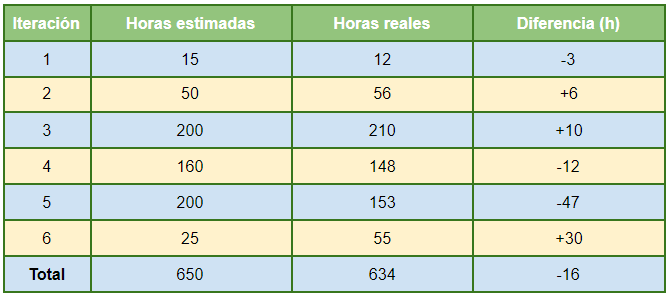
\includegraphics[width=\textwidth]{img/cap4/analisistiempo.jpg}

\clearpage

\section{Costes de desarrollo}
	
\subsection{Costes Directos}	

\textbf{Personal}

Dado que aunque sepamos algo de PHP gracias a algunas asignaturas cursadas anteriormente, no tenemos ninguna experiencia con Angular, calcularemos nuestros sueldos clasificándonos como programadores junior. Dicho conjunto cobra una media de 19.000€ al año, lo cual sería 1.584€ al mes, que al dividirlos en un horario de trabajo de 40 horas semanales, 160 horas al mes, equivaldría a 10€ la hora.\\

Esto hay que multiplicarlo por dos ya que el equipo del proyecto está formado por dos personas, es decir, dos programadores junior con sus respectivos sueldos, por lo que sería un total de 20€ la hora.\\

\subsection{Costes Indirectos}

Realizaremos el proyecto en Microsoft Visual Studio Code, un entorno de desarrollo gratuito, en una base de TypeScript con Angular usando el back-end en PHP a modo de API encargado de realizar las peticiones a una base de datos de MariaDatabase (MySQL), cuyas licencias son gratuitas.\\

Para el almacenamiento de datos en la nube usaremos GitHub y Google Drive, los cuales disponen de licencia gratuita con aspectos limitados.\\

Para la redacción utilizaremos tanto Google Docs como TeXStudio, ambos con licencia gratuita.\\

Para la gestión de tiempo y comunicación usaremos Toggl y WhatsApp respectivamente, las cuales también disponen de licencia gratuita (con limitaciones en el caso de Toggl).\\

Los únicos costes indirectos que podríamos encontrar sería la electricidad y la conexión a Internet, lo cual supone de media 35€ por persona, 70€ en total al mes.\\

\subsection{Amortizaciones}

Para realizar el proyecto hemos usado los siguientes equipos:\\

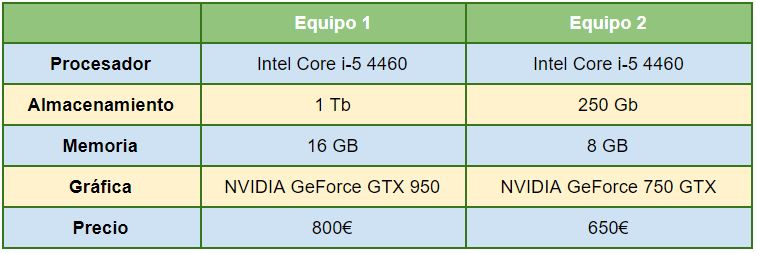
\includegraphics[width=\textwidth]{img/cap4/equipos.jpg}

\bigskip

Además de esto para comunicarnos hemos usado nuestros teléfonos móviles, por eso hemos decidido añadirlo al documento:\\

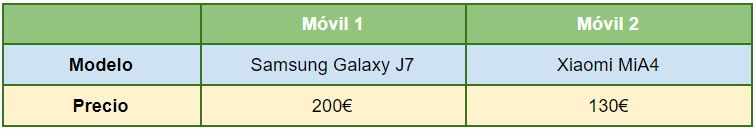
\includegraphics[width=\textwidth]{img/cap4/moviles.jpg}


\subsection{Total}	

Finalmente, sumaremos todos los cálculos anteriores para dar una cifra al precio total:\\

TODO TABLA TOTAL



	

	
     \chapter{An\'alisis de requisitos y dise\~no}\label{requisitos}

\section{Participantes del proyecto}

\bigskip

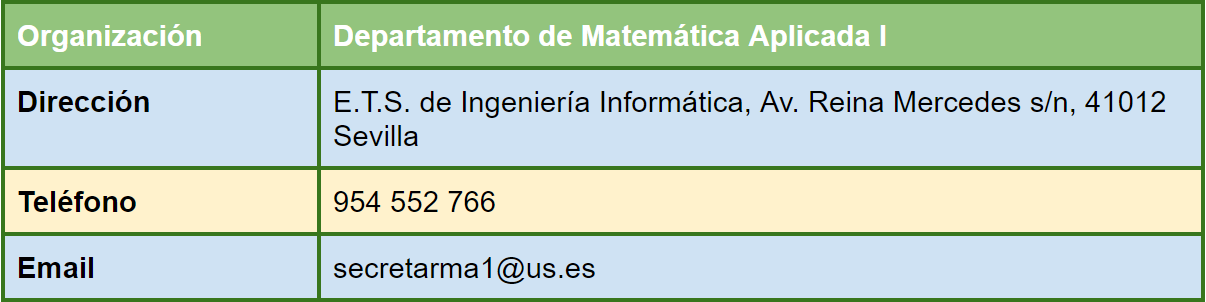
\includegraphics[width=\textwidth]{img/cap5/participantes/1.png}

\bigskip

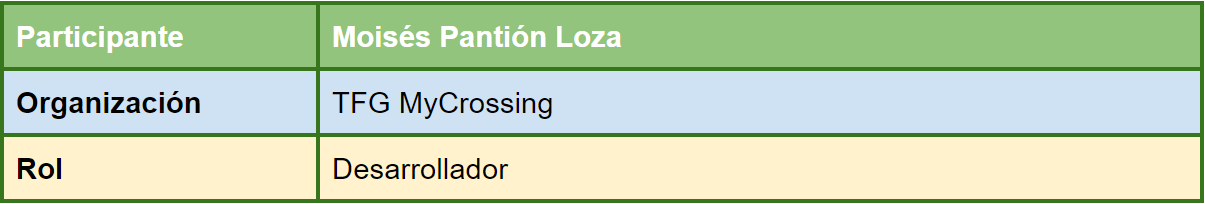
\includegraphics[width=\textwidth]{img/cap5/participantes/2.png}

\bigskip

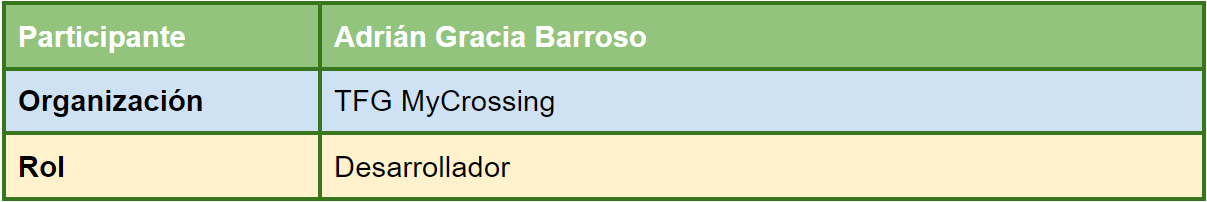
\includegraphics[width=\textwidth]{img/cap5/participantes/3.png}

\bigskip

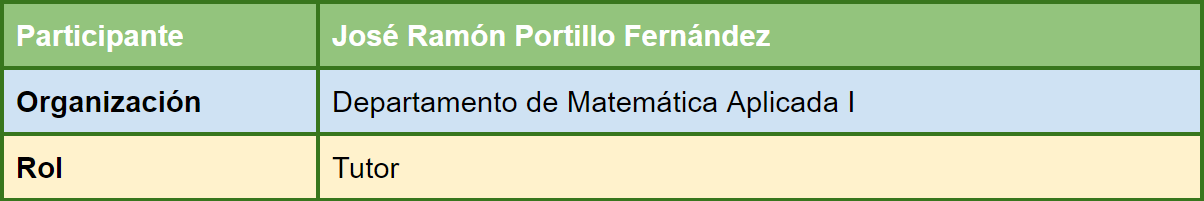
\includegraphics[width=\textwidth]{img/cap5/participantes/4.png}

\bigskip

\section{Requisitos}
	\subsection{Requisitos de Informaci\'on}
	
	\bigskip
	
	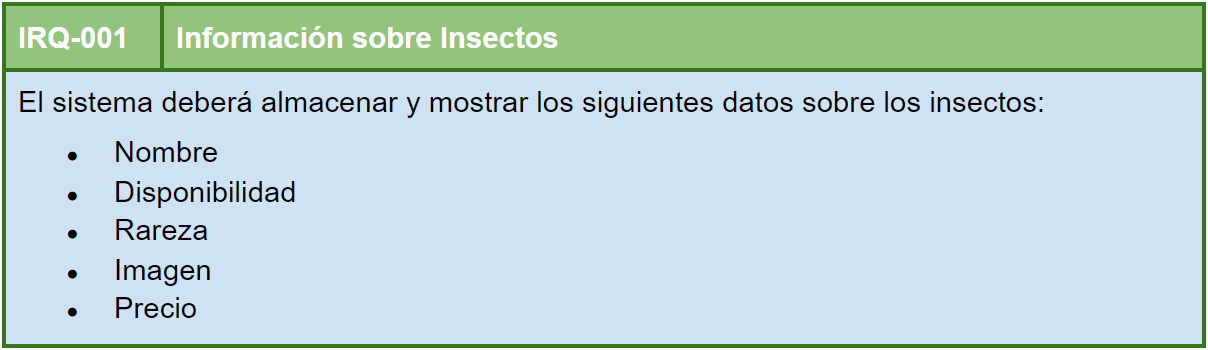
\includegraphics[width=\textwidth]{img/cap5/IR/1.png}
	
	\bigskip
	
	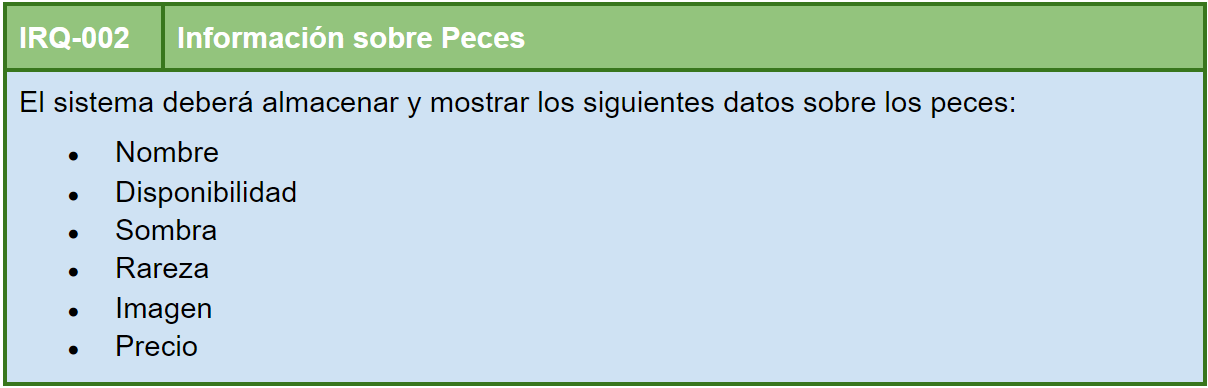
\includegraphics[width=\textwidth]{img/cap5/IR/2.png}
	
	\bigskip
	
	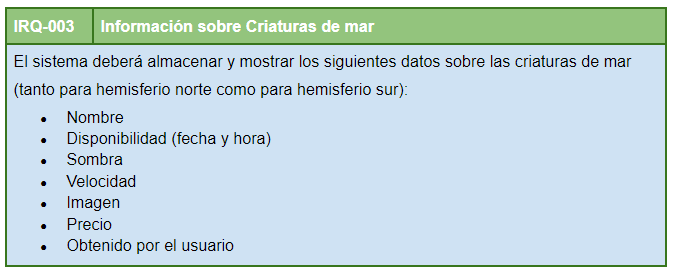
\includegraphics[width=\textwidth]{img/cap5/IR/3.png}
	
	\bigskip
	
	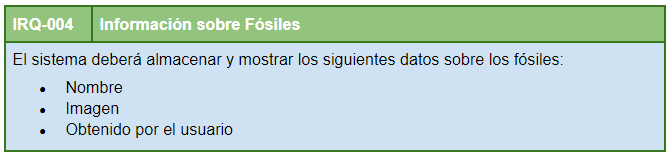
\includegraphics[width=\textwidth]{img/cap5/IR/4.png}
	
	\bigskip
	
	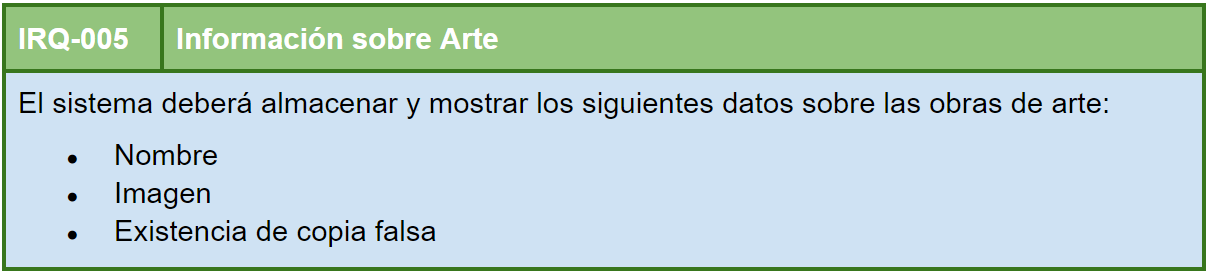
\includegraphics[width=\textwidth]{img/cap5/IR/5.png}
	
	\bigskip
	
	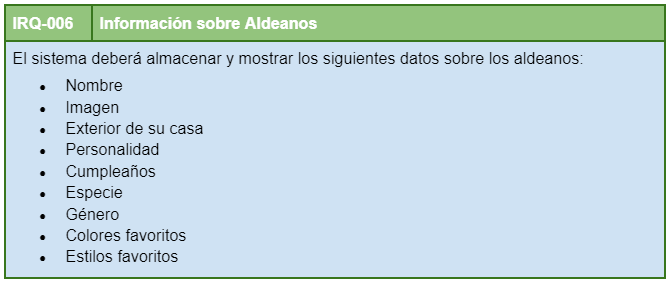
\includegraphics[width=\textwidth]{img/cap5/IR/6.png}
	
	\bigskip
	
	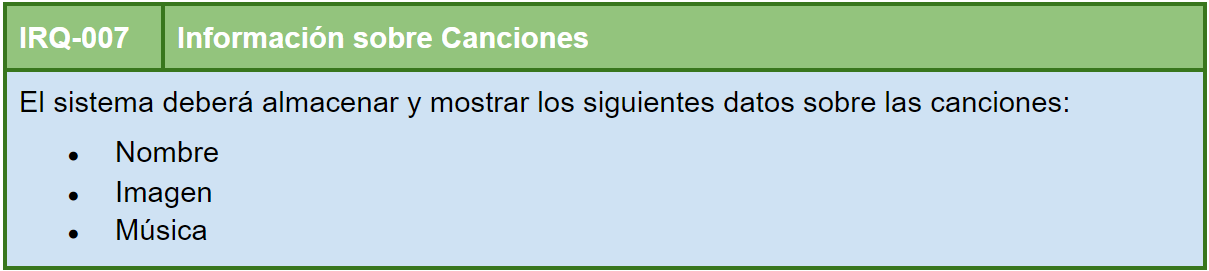
\includegraphics[width=\textwidth]{img/cap5/IR/7.png}
	
	\bigskip
	
	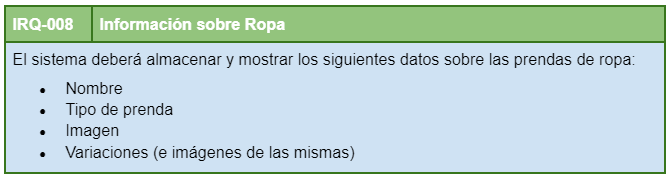
\includegraphics[width=\textwidth]{img/cap5/IR/8.png}
	
	\bigskip
	
	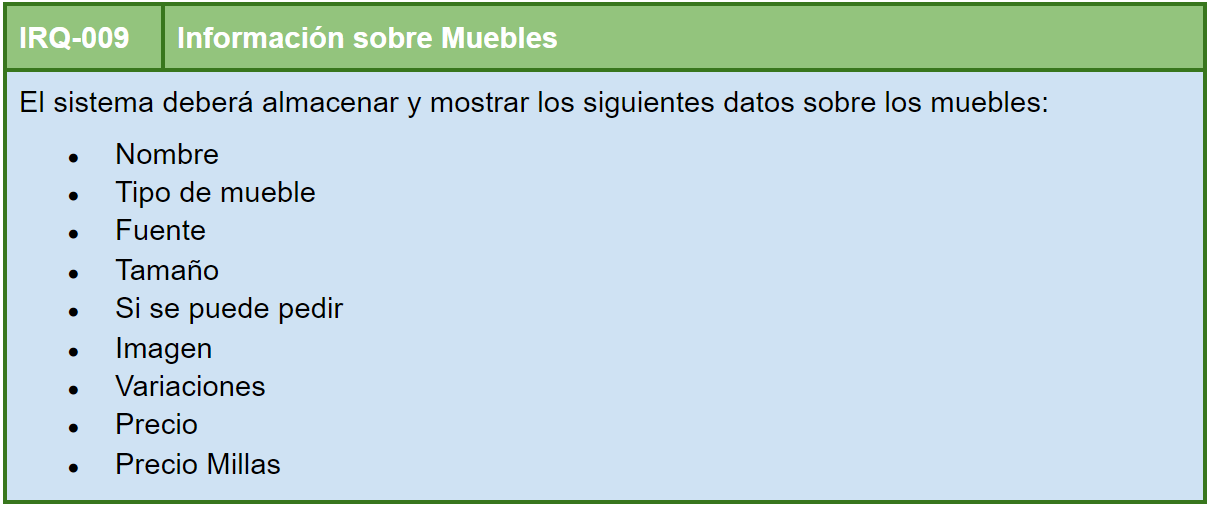
\includegraphics[width=\textwidth]{img/cap5/IR/9.png}
	
	\bigskip
	
	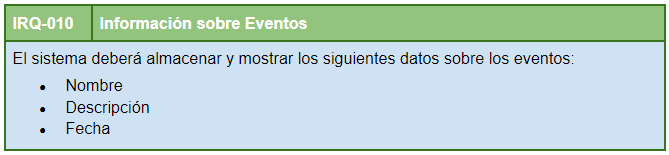
\includegraphics[width=\textwidth]{img/cap5/IR/10.png}
		
	\subsection{Requisitos Funcionales}
	
	\bigskip
	
	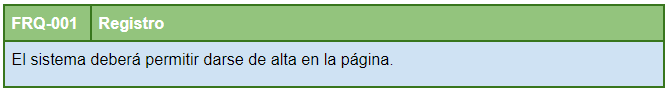
\includegraphics[width=\textwidth]{img/cap5/FR/1.png}
	
	\bigskip
	
	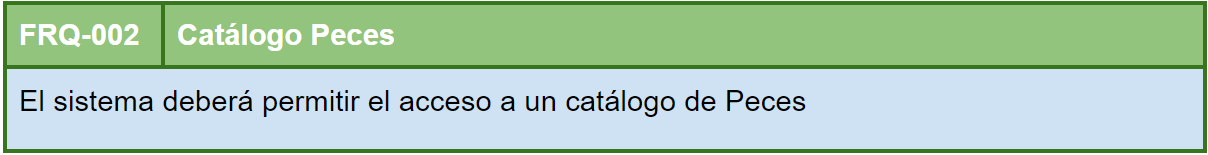
\includegraphics[width=\textwidth]{img/cap5/FR/2.png}
	
	\bigskip
	
	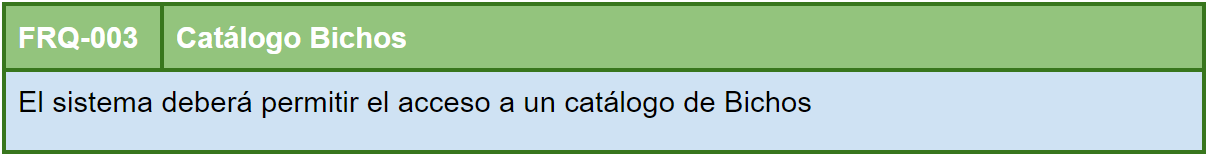
\includegraphics[width=\textwidth]{img/cap5/FR/3.png}
	
	\bigskip
	
	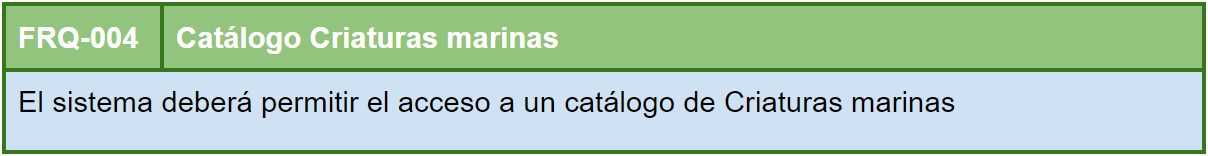
\includegraphics[width=\textwidth]{img/cap5/FR/4.png}
	
	\bigskip
	
	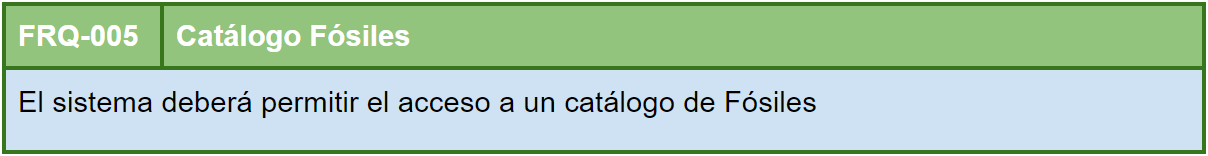
\includegraphics[width=\textwidth]{img/cap5/FR/5.png}
	
	\bigskip
	
	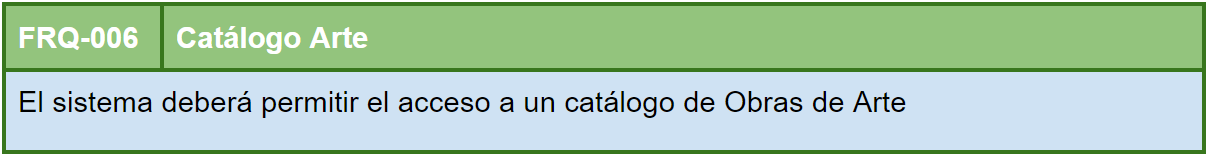
\includegraphics[width=\textwidth]{img/cap5/FR/6.png}
	
	\bigskip
	
	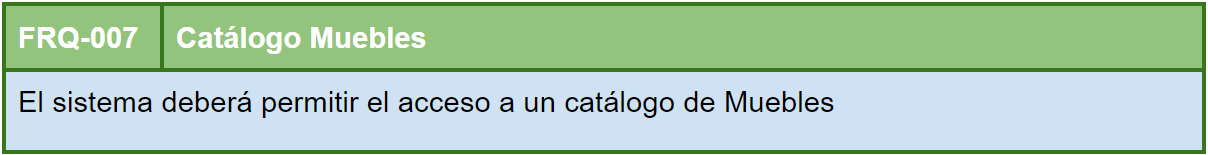
\includegraphics[width=\textwidth]{img/cap5/FR/7.png}
	
	\bigskip
	
	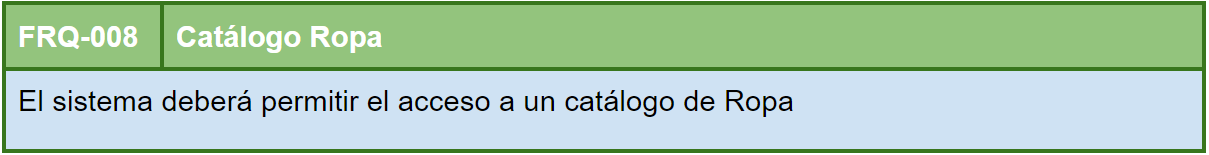
\includegraphics[width=\textwidth]{img/cap5/FR/8.png}
	
	\bigskip
	
	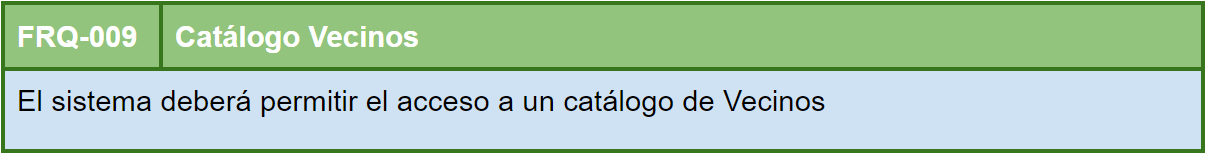
\includegraphics[width=\textwidth]{img/cap5/FR/9.png}
	
	\bigskip
	
	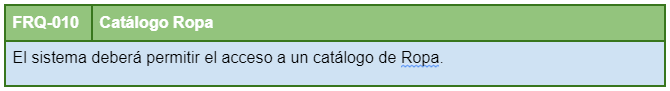
\includegraphics[width=\textwidth]{img/cap5/FR/10.png}
	
	\bigskip
	
	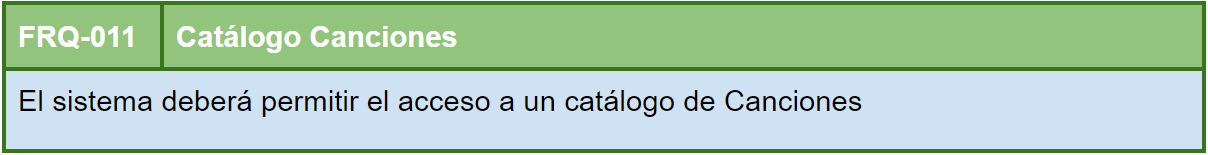
\includegraphics[width=\textwidth]{img/cap5/FR/11.png}
	
	\bigskip
	
	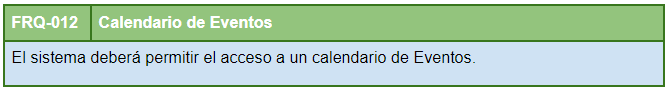
\includegraphics[width=\textwidth]{img/cap5/FR/12.png}
	
	\bigskip
	
	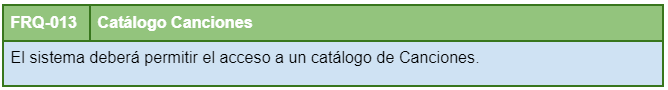
\includegraphics[width=\textwidth]{img/cap5/FR/13.png}
	
	\bigskip
	
	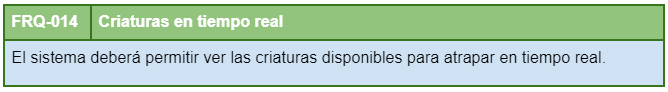
\includegraphics[width=\textwidth]{img/cap5/FR/14.png}
	
	\bigskip
	
	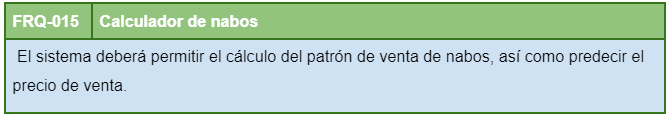
\includegraphics[width=\textwidth]{img/cap5/FR/15.png}
	
	\bigskip
	
	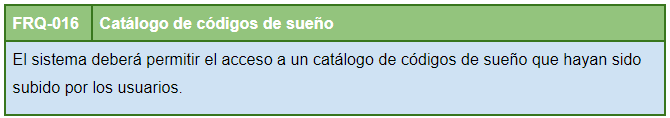
\includegraphics[width=\textwidth]{img/cap5/FR/16.png}
	
	\bigskip
	
	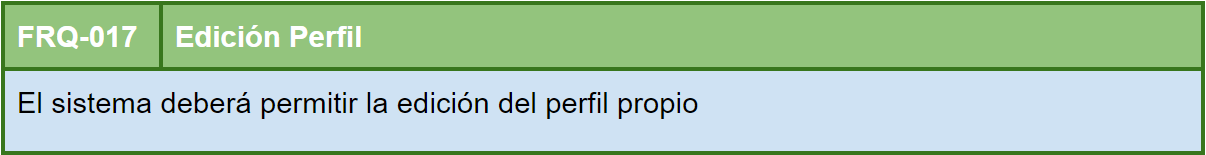
\includegraphics[width=\textwidth]{img/cap5/FR/17.png}
	
	\bigskip
	
	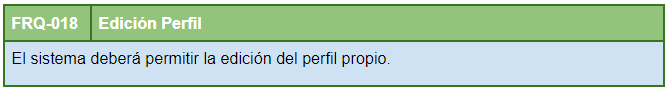
\includegraphics[width=\textwidth]{img/cap5/FR/18.png}
	
	\bigskip
	
	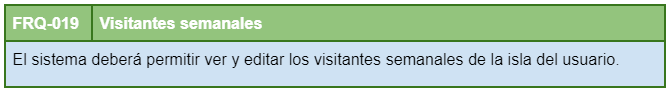
\includegraphics[width=\textwidth]{img/cap5/FR/19.png}
	
	\bigskip
	
	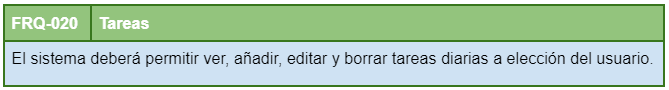
\includegraphics[width=\textwidth]{img/cap5/FR/20.png}
	
	\bigskip
	
	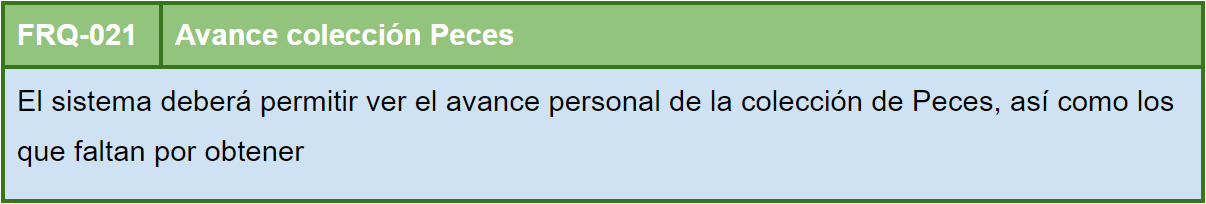
\includegraphics[width=\textwidth]{img/cap5/FR/21.png}
	
	\bigskip
	
	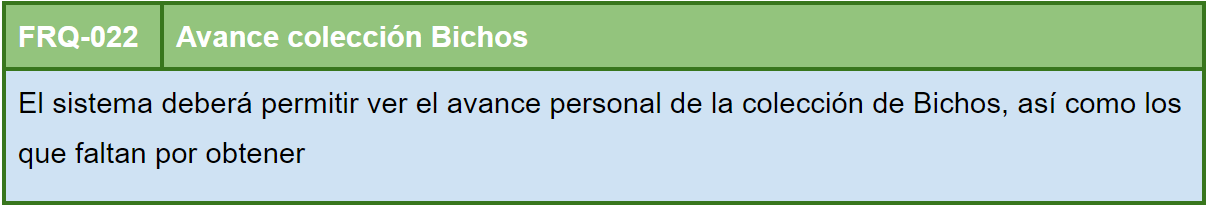
\includegraphics[width=\textwidth]{img/cap5/FR/22.png}
	
	\bigskip
	
	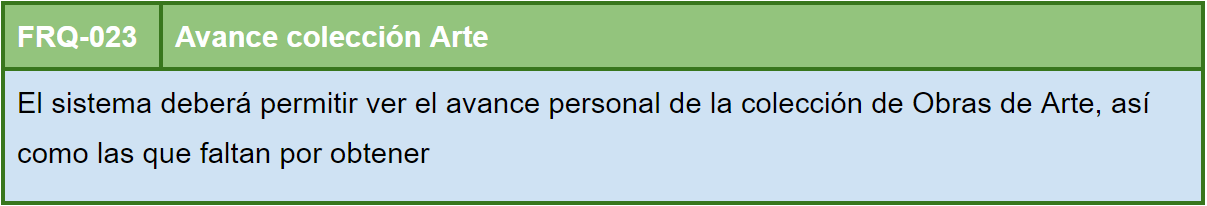
\includegraphics[width=\textwidth]{img/cap5/FR/23.png}
	
	\bigskip
	
	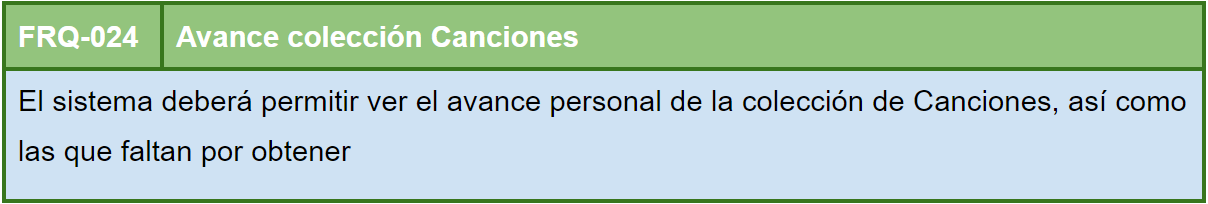
\includegraphics[width=\textwidth]{img/cap5/FR/24.png}
	
	\bigskip
	
	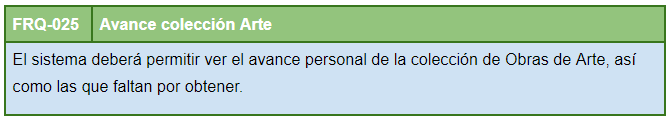
\includegraphics[width=\textwidth]{img/cap5/FR/25.png}
	
	\bigskip
	
	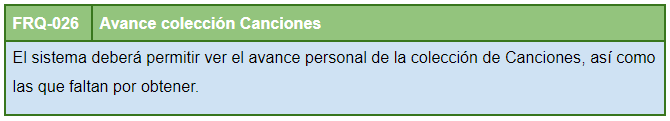
\includegraphics[width=\textwidth]{img/cap5/FR/26.png}
	
	\bigskip
	
	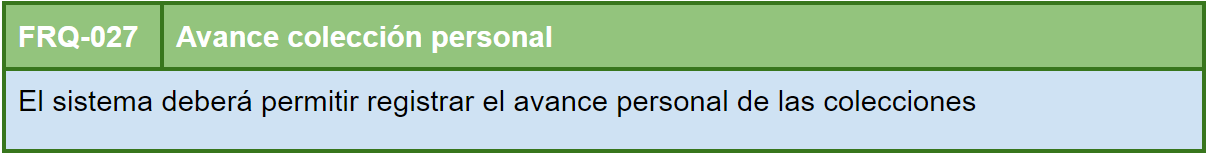
\includegraphics[width=\textwidth]{img/cap5/FR/27.png}
	
	\bigskip
	
	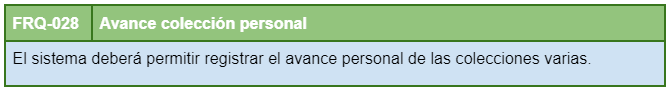
\includegraphics[width=\textwidth]{img/cap5/FR/28.png}
	
	\bigskip
	
	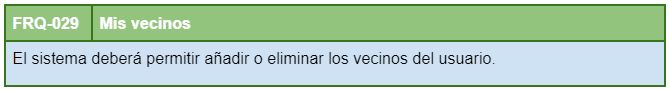
\includegraphics[width=\textwidth]{img/cap5/FR/29.png}
	
	\bigskip
	
	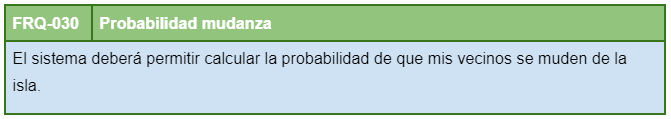
\includegraphics[width=\textwidth]{img/cap5/FR/30.png}

	\subsection{Requisitos no Funcionales}
	
	\bigskip
	
	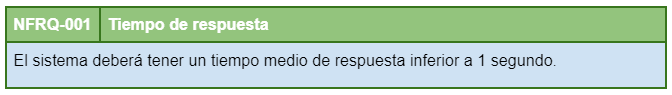
\includegraphics[width=\textwidth]{img/cap5/NFR/1.png}
	
	\bigskip
	
	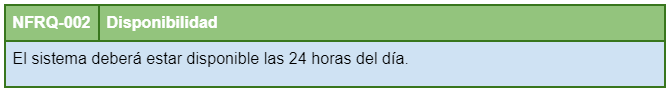
\includegraphics[width=\textwidth]{img/cap5/NFR/2.png}
	
\section{Diagrama de Clases}

	\bigskip

	Dado que tratamos con grandes cantidades de información, gran parte de ella la tenemos que obtener a través de APIs. Así mismo, como sed trata de información de un videojuego, muchos datos han de aparecer en forma de enumeraciones.
	
	\bigskip
	
	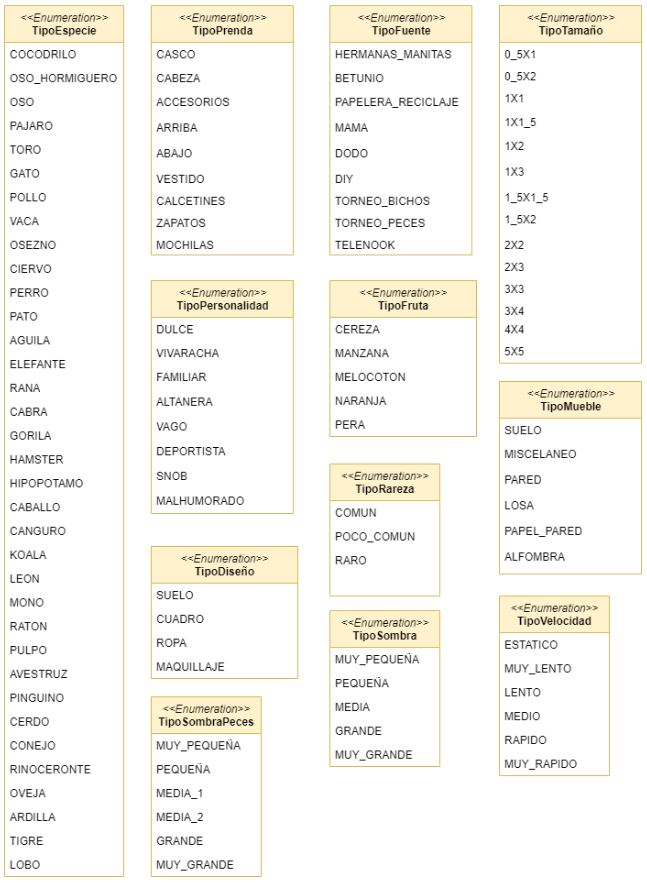
\includegraphics[width=\textwidth]{img/cap5/diagramaclases/enums.jpg}
	
	\bigskip
	
	Debido al gran tamaño del diagrama de clases, vamos a verla dividida en partes más pequeñas de forma que muestren distintas relaciones y se pueda ver de forma más clara.
	
	\bigskip
	
	A continuación se puede ver la clase Museo, la cual recoge la colección personal de Insectos, Peces, Criaturas Marinas, Fósiles y Obras de Arte.
	
	\bigskip
	
	\includegraphics[width=\textwidth]{img/cap5/diagramaclases/museo.jpg}
	
	\bigskip
	
	Luego tenemos la clase Catálogo que de manera análoga hace lo mismo con la Ropa, los Muebles y las Canciones.
	
	\bigskip
	
	\includegraphics[width=\textwidth]{img/cap5/diagramaclases/catalogo.jpg}
	
	\bigskip
	
	Tanto Museo como Catálogo van asociados a Usuario, así como Vecinos y Diseños.
	
	\bigskip
	
	\includegraphics[width=\textwidth]{img/cap5/diagramaclases/usuario.jpg}
	
	\bigskip

	Por último está la clase Evento que no está relacionada con ninguna otra, ya que solo se usarán los datos para el Calendario de Eventos el cual es meramente informativo.
	
	\bigskip
	
	\begin{center}
		\includegraphics[width=6cm]{img/cap5/diagramaclases/evento.jpg}
	\end{center}
\section{Dise\~no}

A continuación ofrecemos una primera visión de lo que sería la interfaz gráfica del sistema, acompañado de algunas explicaciones para entender a priori el funcionamiento  del sistema, ya que entraremos en detalle más adelante en el manual de usuario. En las imágenes aparecen anotaciones realizadas en rojo para el mejor entendimiento del estilo que se busca obtener de cara a la hora de implementar las vistas.\\

Empezando por la página de inicio (v\'ease la figura~\ref{fig:inicio1}), tendríamos el navegador en la zona superior para acceder a las diferentes secciones del sistema que no necesitan que el usuario se haya registrado, además de un botón para iniciar sesión en caso de que se disponga de una cuenta en la página.\\

\figura{0.8}{img/mockups/Inicio - 1.png}{Inicio 1}{fig:inicio1}{}


Bajando vemos diferentes secciones, disponiendo en primer plano de la portada con un botón para acceder al registro. Más abajo se encuentran las diferentes secciones de enciclopedia con las que contará el sistema: peces, bichos, criaturas marinas, fósiles y obras de arte (v\'ease la figura~\ref{fig:inicio1}), así como del catálogo de muebles, ropa, vecinos e incluso un calendario de eventos {(v\'ease la figura~\ref{fig:inicio2})}.\\

\figura{0.8}{img/mockups/Inicio - 2.png}{Inicio 2}{fig:inicio2}{}

Empezando por las secciones que hemos comentado en el párrafo anterior, a continuación tenemos un listado de peces, aunque el formato es genérico para los demás listados, cambiado algunos pequeños detalles en cada uno como ciertos filtros.\\

Podemos observar que arriba se encuentra la sección de filtros para que el usuario pueda realizar una búsqueda más específica de manera simple. Debajo de los filtros se encuentra el listado en sí, que muestra una recopilación de los peces (en este caso) disponibles en el juego. Cada item cuenta con una imagen, su nombre y algunos de los datos más relevantes, como precio de venta o localización, y si se hace clic en la celda se abre un menú con información más detallada, de forma que lo importante esté siempre a la vista y no haya que entrar en los menús de forma repetitiva.\\
 
En rojo se muestran aquellas criaturas que no se encontrarán disponibles el mes que viene, y además, si el usuario está registrado en el sistema y ha iniciado sesión, puede llevar recuento de los que ya ha capturado marcándolos con el tick superior derecho en cada item, cambiándose así el fondo a un color distinto para diferenciarlos a simple vista {(v\'ease la figura~\ref{fig:listado})}.\\

\figura{1}{img/mockups/Listado.png}{Listado genérico}{fig:listado}{}

Para terminar con el contenido de la página de inicio (ya que a excepción del calendario, lo demás son todo listados como el que acabamos de ver), tendríamos el calendario de eventos {(v\'ease la figura~\ref{fig:eventos1})}.\\

\figura{0.8}{img/mockups/Eventos - 1.png}{Eventos}{fig:eventos1}{}

Esta sección no es mas que un gran calendario donde el usuario puede ver tanto las festividades del juego como los cumpleaños de los vecinos. Sin embargo, dispondrá de información adicional para los eventos al hacer clic en ellos, de forma que se desplegará un menú {(v\'ease la figura~\ref{fig:eventos2})} en el que podremos ver información útil de dicho evento, como visitantes, objetos temáticos, actividades especiales, etc. De esta forma el usuario puede tener una idea general de todo lo que se puede hacer en ese evento y planificarse mejor su agenda.\\

\figura{0.8}{img/mockups/Eventos - 2.png}{Eventos - Detallado}{fig:eventos2}{}

Una vez acabado con el contenido de la página principal, si el usuario quisiera registrarse accedería a la siguiente vista {(v\'ease la figura~\ref{fig:registro})}, la cual es una simple página de registro con información relevante al juego, como el nombre de la Isla, el tipo de fruta o la localización. Este último es bastante importante ya que dependiendo de si se encuentra en el hemisferio norte o sur, el usuario visualizará unos datos u otros.\\

\figura{1}{img/mockups/Registro.png}{Registro}{fig:registro}{}

Si se completa el registro de forma satisfactoria, se puede acceder al perfil del usuario, el cual dispone de varias secciones {(v\'ease la figura~\ref{fig:perfil})}.\\

\figura{0.8}{img/mockups/Perfil.png}{Perfil}{fig:perfil}{}

A la izquierda se muestra la información del usuario a modo de resumen o biografía. A la derecha se encuentra la sección que se usará de forma diaria. Por una parte tenemos las tareas, las cuales se pueden editar con un icono dependiendo del propósito que tengan y serán marcadas por el usuario una vez hayan sido realizadas, reiniciándose cada día. Por otra parte tenemos la lista de visitantes semanales, donde podremos observar los visitantes de la semana anterior e ir rellenando los de esta semana en consecuencia.\\

Si bajamos, encontraremos un listado de los vecinos que actualmente residen en nuestra isla, con posibilidad de ir añadiendo hasta un máximo de diez vecinos. Al colocar el cursor sobre cualquiera de ellos, se mostrará información sobre el mismo.\\

Más abajo tenemos un pequeño listado de algunas colecciones de objetos especiales para que el usuario lleve un recuento de las que ya dispone y las pueda localizar de una manera más sencilla y organizada. Las colecciones irán variando dependiendo de que botón se encuentre activo, y dispondrá de un recuadro de texto para realizar una búsqueda específica.\\

Por último, tenemos una sección de galería que sirva a modo de portfolio para el usuario, para tener todas las capturas y/o vídeos recopilados en un mismo sitio.\\

Una vez acabado con el perfil, pasamos a las tres últimas vistas que se encuentran en el navegador principal de la página. Primero encontramos una página que es una recopilación de listados (como el mencionado anteriormente) de bichos, peces y criaturas marinas. La diferencia, aparte de encontrarse los tres juntos, es que en este listado aparecen todas las criaturas que se pueden atrapar actualmente, actualizándose a medida que lo hace el tiempo {(v\'ease la figura~\ref{fig:cazarahora1})}. Esto es útil ya que si un usuario quiere saber que criaturas puede cazar ahora en su isla, tan solo tiene que acceder a esta página y ya dispone de dicha información, sin registro ni pérdida de tiempo, ya que dispone de las tres colecciones de criaturas en la misma página.\\

Además, también dispone de una serie de filtros para realizar una búsqueda algo más específica, incluso con opciones de ocultar cierta información para evitarse así los "spoilers", de forma que sepa donde puede encontrar la criatura pero no sepa ni cuál ni cómo es, de esta forma puede tener una cierta ayuda a la hora de capturarla pero seguir teniendo la emoción de no saber que es lo que le aguarda.\\

\figura{0.8}{img/mockups/Cazar Ahora - 1.png}{Cazar ahora 1}{fig:cazarahora1}{}

\figura{0.8}{img/mockups/Cazar Ahora - 2.png}{Cazar ahora 2}{fig:cazarahora2}{}

A continuación tendríamos la calculadora de nabos. En esta página se proporciona un poco de información acerca del mercado de nabos dentro del juego, de forma que el usuario entienda algo mejor como funciona y los distintos patrones de venta que existen {(v\'ease la figura~\ref{fig:nabos})}.\\

En la parte inferior se encontraría la calculadora en sí, donde el usuario debe de escribir la información que haya ido recopilando para poder así realizar una predicción del patrón que hay actualmente en su isla. Además se acompañará de una gráfica y una tabla de precios por si quisiera información más detallada.\\

\figura{0.8}{img/mockups/Nabos.png}{Calculadora de Nabos}{fig:nabos}{}

Para terminar con este apartado y con el capítulo, por último veremos la vista del probador. Esta es una de las funcionalidades que crearemos y que consiste, como su propio nombre indica, en un probador de ropa {(v\'ease la figura~\ref{fig:probador})}.\\

En el centro tendremos una imagen de nuestro personaje, al cual podremos personalizar utilizando el menú superior, actualizándose a medida que seleccionemos las distintas opciones. Una vez elegido el personaje, la página dispondrá de un catálogo de ropa dividido en secciones (cabeza, torso, accesorios etc) para que el usuario pueda buscar la prenda que quiera probarse. Una vez la encuentre, con un clic sobre la prenda, esta aparecerá sobre el personaje central. Además se mostrarán en un desplegable todas las variaciones de color de las prendas para obtener así un catálogo completo. De esta forma el usuario puede realizar combinaciones de ropa para probar nuevos estilos y decidir que prendas necesita, en vez de ir comprándolas en el juego para luego cambiar de opinión.\\

\figura{0.8}{img/mockups/Probador.png}{Probador}{fig:probador}{}



 
     \chapter{Implementaci\'on}\label{implementacion}

\section{Entorno de desarrollo}

\figura{0.25}{img/cap6/vscode.png}{Logotipo Visual Studio Code}{fig:vscode}{}
El entorno de desarrollo utilizado para estra proyecto ha sido Microsoft Visual Studio Code, ya que es un IDE bastante versátil que soporta una gran variedad de lenguajes y que, al ser de código abierto, presenta la posibilidad de instalar plugins creados por la comunidad para obtener funcionalidades útiles para cualquier tipo de lenguaje. Dado que vamos a trabajar con Angular, con la instalación de un paquete de plugins de Angular hemos podido trabajar de forma bastante cómoda y sin ningún problema.\\

Además, ofrece soporte para Git, de forma que se pueden realizar operaciones en el repositorio de forma bastante sencilla, así como gestionar lo posibles errores que puedan surgir mediante la misma interfaz, por lo que resulta bastante cómodo.\\

La principal ventaja de Visual Studio Code es que, al ser un IDE universal, contamos con varias funciones generales de los IDE (debug, consola de comandos) pero aplicado a una gran variedad de lenguajes, de forma que con el simple hecho de tenerlo instalado ya se puede comenzar a trabajar (incluso sin la necesidad de plugins, aunque no es recomendable). Es por esto que con el simple hecho de disponer del IDE y descargar un par de plugins, ya se puede trabajar de forma cómoda, y además se puede adaptar de manera sorprendente ya que, si en algún momento hay que trabajar con otro lenguaje, se puede realizar perfectamente sin tener que descargar otro IDE. Directamente desde Visual Studio Code y con algun plugin extra, ya se puede incorporar el nuevo lenguaje y trabajar de forma cómoda con ambos, lo cual centraliza el trabajo en una misma aplicación y resulta más eficiente.\\

\section{Tecnolog\'ias utilizadas}

La idea principal de este proyecto era usar Angular como tecnología para el front-end por las razones ya explicadas anteriormente. Las demás tecnologías que fueramos a usar no iban a tener tanto peso para nosotros como lo iba a tener esta, por lo que ibamos con la mente abierta dispuestos a usar la tecnología que, además de adaptarse bien a nuestro proyecto, fuera compatible con Angular. Al principio, pensamos en usar una base de Spring para el back-end, ya que es un framework que hemos visto en la carrera y además hemos adquirido experiencia en Java durante todo la carrera, pero debido a que no sabíamos nada sobre el funcionamiento de Angular (y todo lo que puede llegar a abarcar), pensamos que el peso de la aplicación se la llevaría el back-end (en Spring al principio). Sin embargo, una vez aprendimos y nos pusimos a dar nuestros primeros pasos en el framework, descubrimos que se puede realizar la gran mayoría de funcionalidades de la aplicación en Angular.\\

Además luego llegó la hora de conectar el proyecto en Angular con la base de datos. Estábamos acostumbrados a Spring, que realiza toda la gestión de base de datos por detrás en el mismo framework y tan solo es necesario inicializar los repositorios con las querys, así como las beans para popular la base de datos. Sin embargo, al estar trabajando con Angular, tuvimos que buscar información sobre como realizar esta conexión y descubrimos que se podía conectar a una base de datos gestionada mediante PHP con una simple petición HTTP al archivo que realizase la conexión y las operaciones oportunas. Esta idea nos gustó bastante ya que, no solo tendríamos que usar otro lenguaje (por lo que aprendemos más), sino que además podíamos utilizar la conexión con la base de datos a modo de API, haciendo peticiones HTTP desde Angular al correspondiente archivo PHP, el cual se encarga de abrir la conexión con la base de datos, realizar la consulta oportuna, y devolver los datos, los cuales Angular se encarga de recoger, transformarlos en caso de ser necesario, y finalmente, mostrarlos.\\

Es por esto que decidimos entonces usar XAMPP, ya que ofrece un servidor de Apache (en el cual se ejecutarían los archivos PHP que se encargasen de conectarse con la base de datos) así como una base de datos de MariaDatabase. Esto nos vino particularmente bien ya que en otras asignaturas habíamos usado XAMPP, y no solo eso sino que la base de datos de MariaDatabase esta basada en MySQL, que es el lenguaje que hemos dado durante toda la carrera, por lo que al estar trabajando ya con dos lenguajes que no conocemos del todo, uno familiar se recibe bastante bien.\\

Una vez montada la estructura de la base de datos y habiendo probado ya el funcionamiento de Angular y todo su alcance, nos dimos cuenta de que el back-end de Spring que habíamos pensado no era para nada necesario, ya que toda la lógica se realiza a través de este framework y las operaciones para obtener datos de la base de datos las íbamos a realizar con PHP, por lo que al final se descartó la idea de usar Spring como framework para el back-end ya que contábamos con todo lo que necesitábamos con la estructura que disponíamos.\\

\clearpage

\subsection{Angular}

\figura{0.4}{img/cap6/angular.png}{Logotipo Angular}{fig:angular}{}
Angular es un framework para aplicaciones web desarrollado en TypeScript de código abierto que suele ser utilizado para la creación de aplicaciones web de una sola página (SPA), además de seguir el diseño Modelo-Vista-Controlador (MVC).\\

Angular funciona mediante componentes, los cuales disponen de sus respectivas variables y métodos que se encargan de realizar la lógica, así como de operar con su vista asociada. De esta forma, obtenemos pequeños paquetes de código, cada uno con su vista y su lógica. Podría explicarse como si de un puzzle se tratase, pero con muchas posibles soluciones, siendo cada pieza un componente con su vista, sus variables y métodos. Cada pieza es funcional por si misma, pero el objetivo es juntarlos con otros componentes para obtener la aplicación (o vista) completa.\\

Además de ser una forma bastante interesante de desarrollar una aplicación, es una muy buena forma de evitar la repetición de código, ya que si se necesita reusar un componente es tan fácil como importarlo y se encuentra listo. De la misma forma, se trabaja con servicios, directivas y etiquetas que pueden ser reutilizadas, reduciendo así la carga de trabajo considerablemente y aumentando la limpieza del código.\\

Además, una vez se esté ejecutando la aplicación, esta se actualiza con los nuevos cambios que se realicen, algo que resulta bastante cómodo a la hora de realizar algunas pruebas dado que no hay que estar ejecutando constantemente la aplicación.\\

\clearpage

\subsection{XAMPP y Apache}

\figura{0.6}{img/cap6/xampp.png}{Logotipo XAMPP}{fig:xampp}{}
XAMPP es un paquete de software libre que consiste en el sistema de gestión de bases de datos de MySQL, el servidor web Apache y los intérpretes para PHP y Perl.\\

Es una opción bastante buena para nuestro proyecto ya que resulta bastante sencillo de usar y ademas nos proporciona tanto el servidor web como la base de datos y el interprete para PHP, todo desde una misma aplicación.\\

\figura{0.7}{img/cap6/apache.png}{Logotipo Servidor Web Apache}{fig:apache}{}
El servidor web de Apache es un servidor HTTP de código abierto multiplataforma con una arquitectura basada en módulos. Tiene una sección base que actúa como núcleo, y a esta base se le adjuntan módulos que aportan funciones básicas para el servidor web. Además, existen módulos externos para ampliar su funcionalidad, ya sea ofreciendo soporte para distintos lenguajes (Perl, Python, PHP y Ruby entre otros) u ofreciendo otras funciones como llevar un control del tráfico web.\\

\clearpage

\subsection{PHP}
\figura{0.4}{img/cap6/php.png}{Logotipo PHP}{fig:php}{}

PHP es un lenguaje de programación libre especialmente adaptado para el desarrollo web y está orientado al desarrollo de aplicaciones web dinámicas con acceso a información almacenada en una base de datos. Funciona del lado del servidor, por lo que el código es invisible al navegador y al cliente, ya que es el servidor el encargado de ejecutar el código y enviar el resultado  HTML al navegador.\\

El código suele ser procesado en un servidor web por un intérprete PHP implementado como un módulo, y el resultado es representado mediante una petición HTTP. Es bastante versátil ya que puede ser desplegado en la mayoría de servidores web y en todos los sistemas operativos y plataformas sin coste alguno. Gracias a que es libre y a su flexibilidad, es uno de los lenguajes mas populares como base para las aplicaciones web.\\

Su alcance es bastante amplio, ya que puede utilizarse insertando su código en archivos HTML, como para operar con bases de datos o incluso actuar como servicio REST. Es por esto que posee gran capacidad de conexión con la mayoría de motores de base de datos actuales (especialmente con MySQL y PostgreSQL).\\

\clearpage

\subsection{MariaDB y MySQL}

\figura{0.4}{img/cap6/mariadb.png}{Logotipo MariaDatabase}{fig:mariadb}{}

MariaDB es un sistema de gestión de bases de datos derivado de MySQL con licencia GPL. Tiene una alta compatibilidad con MySQL (posee las mismas órdenes, interfaces, API y bibliotecas).\\

\figura{0.4}{img/cap6/mysql.png}{Logotipo MySQL}{fig:mysql}{}

Respecto a MySQL, es un sistema de gestión de base de datos relacional considerada la base de datos de código abierto más popular del mundo. Si MariaDB era un sistema derivado con licencia GPL, MySQL está desarrollado bajo licencia comercial por parte de Oracle.\\

Su uso principal es orientado a aplicaciones web debido a la rapidez que posee a la hora de la lectura de datos. Además, al ser tan popular nos garantiza una gran base de información sobre posibles errores que podamos tener.\\

\clearpage

\subsection{Git}

\figura{0.4}{img/cap6/git.png}{Logotipo Git}{fig:git}{}

Git es un software de control de versiones. Su propósito es llevar registro de los cambios en archivos, incluyendo la coordinación del trabajo que se realiza sobre archivos compartidos entre varias personas. A raíz de este software han surgido plataformas como GitHub o GitDesktop, todo enfocado a la gestión visual y sencilla de las funcionalidades que ofrece Git, así como el alojamiento de proyectos que utilicen dicho sistema de control de versiones.\\

Es uno de los software de control de versiones más populares, lo que ha provocado que muchas aplicaciones ofrezcan compatibilidad con Git, como puede ser Microsoft Visual Studio Code o Eclipse IDE por ejemplo.\\

Como ya se ha comentado, a raiz de Git nació GitHub, siendo también de las plataformas más populares para el alojamiento de proyectos y colaboración simultánea en los mismos. GitHub ofrece desde su servicio básico de alojar proyectos, hasta wikis por cada proyecto, tableros estilo Kanban, gráficas del trabajo y gran cantidad de adiciones para facilitar el trabajo colaborativo en dichos proyectos.\\

Además existen plugins que añaden funcionalidades a la plataforma o que la integran en otras aplicaciones para que su uso esté mas centralizado y sea más cómodo.\\

\clearpage

\section{Dificultades encontradas y soluciones propuestas}

Como es común en todos los proyectos, a medida que se ha ido avanzando en el desarrollo nos hemos ido encontrado con varios obstáculos (unos más grandes que otros) que nos han obligado a desviarnos un poco y buscar soluciones para poder continuar. A continuación se encuentran los obstáculos más significativos y cómo los hemos ido resolviendo:

\subsection{It. 3 - Perfil}

Esta ha sido la primera iteración en la que hemos empezado a programar y hemos desarrollado features. Al principio, dado que íbamos a trabajar con una API de la que sacaríamos todos los datos, pensamos que el perfil del usuario, así como las distintas funciones que habían dentro de este, no resultarían un gran trabajo ya que trataría más de consumir información y que, por lo tanto, sería un buen comienzo para empezar a iniciarnos en Angular.\\

Sin embargo, cuando nos pusimos a desarrollar código, vimos que no era tan simple y que todo lo que pensábamos que sería consumir información, eran en realidad features que había que realizar, con sus respectivos servicios, clases y lógica, ya que necesitábamos almacenar dicha información relacionándola con el usuario. Esto hizo que se aumentara bastante la carga de trabajo, así que para no cargarnos mucho en esta primera iteración de desarrollo, decidimos dejar la implementación de la API para el siguiente sprint (asi como la realización de los tests, ya que no tiene sentido desarrollar unos tests para features que no estan completas).\\

De este modo, aunque algo más laborioso de lo que se pensó en un principio, pudimos realizar un sprint de introducción al lenguaje (del que hemos aprendido bastante) que nos sirve como base para los siguientes sprint, ya que con cada feature que hemos ido desarrollando, hemos descubierto más y más sobre el framework, adquiriendo así las nociones necesarias para avanzar de forma eficiente.

\subsection{It. 3 - Mantener sesiones}

En esta iteración decidimos repartir las tareas de forma que uno de nosotros empezara implementando todo lo relacionado con el registro y el inicio de sesión mientras que el otro se iba encargando de otras tareas, en este caso, de las funciones dentro del perfil.\\

El problema comenzó con lo mencionado en el punto anterior: se combinó el aumento de carga de trabajo con las dificultades que encontramos a la hora de mantener una sesión en la página, ya que era necesario para la mayoría de tareas del perfil. Además, como el servidor de Apache donde se encuentra la base de datos y el servidor de Node.JS en el que se ejecuta Angular están localizados en puertos distintos, no se podía realizar una sesión de forma normal (al igual que muchas otras funciones de PHP como acceder a los datos de una operación POST mediante la variable por defecto de PHP).\\

Esto ocasionó que tuviéramos que dar un rodeo buscando posibles soluciones hasta dar con la actual, que se basa en almacenar un código de verificación que se borre exclusivamente al cerrar sesión, de forma que se mantiene la sesión mientras el usuario tenga asignado un código de verificación que no sea nulo. Debido a este rodeo y al tiempo que llevó tanto encontrar la solución como su implementación, hubo cierta dependencia entre tareas, lo que ocasionó un ligero aumento del tiempo inicial pensado para dichas tareas.

\subsection{It. 3 - Features del perfil}

En la feature de ``Mis vecinos``, teníamos que calcular el porcentaje que tiene cada vecino de mudarse de isla, dependiendo de la amistad que tenga con el jugador y de ciertos parámetros que hayan podido ocurrir. Este algoritmo pensábamos que ya lo habrían sacado del juego y podríamos acceder a él, sin embargo no fue así.\\

Dado que no se había publicado el algoritmo, tuvimos que realizar cierta investigación para dar con la fórmula que calcula dicha probabilidad y acto seguido, implementar nosotros el algoritmo (Agradecimientos al usuario de Twitter \textit{Ninji} que publicó la lógica y las matemáticas que sigue el juego para calcular la probabilidad de mudanza, información a partir de la cual pudimos implementar el algoritmo).\\

Respecto a la feature de ``Colecciones Especiales``, dado que no nos habíamos informado tanto como debíamos sobre la API que íbamos a usar, descubrimos que dicha API no tiene ningún método de filtro mas que obtener objetos por su id, por lo que nos obligaba a hacer una petición con todos los objetos e ir filtrando por ``fuente`` (colección) para seleccionar los que nos interesaban. Esto era posible pero suponía un gran coste computacional, especialmente si lo implementamos de forma que cualquier usuario pueda hacer dicha petición.\\

Ante este problema, dimos con la idea de crear un usuario administrador (el cual no había hecho falta hasta ahora) que pudiera ejecutar dicha petición para actualizar el catalogo de colecciones, de forma que con una sola petición por parte del administrador, se actualizan los items disponibles para los usuarios, de forma que estos acceden a una tabla de la base de datos con datos mínimos (fuente e id).\\

De esta forma, aunque guardamos algunos datos en la base de datos, nos ahorramos tanto el realizar peticiones de forma constante en la que recibimos cientos de objetos, como el filtrarlos para poder obtener los deseados, aumentando así la velocidad de respuesta.

\subsection{It. 4 - API incompleta}

En la iteración 4 debíamos hacer un repaso por las features realizadas en la iteración anterior de forma que añadiésemos todo lo necesario relacionado con la API que íbamos a utilizar para acceder tanto a imágenes como a datos del juego.\\

Sin embargo, una vez nos pusimos a implementar la API \cite{acnhapi}, nos dimos cuenta de que, aunque bastante completa para algunos aspectos del juego, para otros no estaba tan completa y carecía de muchos datos que necesitábamos. Además solo implementaba métodos para obtener o todo el listado de datos, o uno solo (mediante su ID), pero en ningún momento nos dejaba filtrar, por lo que iba a ser un trabajo que íbamos a tener que realizar a mano y que además sería bastante costoso computacionalmente hablando.\\

Es por eso que realizamos otra búsqueda en la web para encontrar una solución distinta que nos proporcionase todo lo que necesitábamos. Primero encontramos otra API \cite{nookipediaapi} que, aunque disponía de más métodos y alguna información que nos podía resultar útil, estaba aun a mitad de desarrollo, por lo que también estaba algo incompleta. Se pensó en implementar ambas API, pero el resultado no era lo que buscábamos, era una solución algo compleja y no nos convencía del todo, pero parecía ser la única opción.\\

Sin embargo, tras seguir buscando encontramos una librería \cite{acnhnpm} que se podía instalar directamente en Angular que disponía de toda la información que necesitábamos, así como ciertas traducciones e imágenes, por lo que decidimos usar esta librería ya que, no solo nos daba todo lo que necesitábamos sino que ademas su uso era extremadamente sencillo. 

\subsection{It. 5 - Código reciclado}

En la iteración 5 introdujimos la calculadora de nabos y el calendario de eventos entre otras features. Para la calculadora necesitábamos el algoritmo que calculaba los precios establecidos en el juego. Dicho algoritmo había sido datamineado por un usuario ya mencionado anteriormente en esta memoria, Ninji \cite{nabosninji}.\\

El problema surge a raíz de que dicho algoritmo, que se encuentra subido en la plataforma GitHub, estaba para otro lenguaje distinto al de nuestro proyecto, por lo que no pudimos usarlo directamente. Al principio consideramos intentar adaptarlo, pero era tan extenso y complejo que no merecía la pena dedicarle tantas horas a esa tarea, por lo que optamos por otra solución.\\

De entre varias webs que ya disponen de esta herramienta, hay una \cite{turnipprophet} que está realizada al completo en JavaScript, por lo que se realiza todo el trabajo por parte del cliente. Investigando descubrimos que dicho código también se encontraba en GitHub bajo la licencia de Apache 2.0, la cual nos permite usar el código mientras que cumplamos ciertas reglas, por lo que decidimos usar lo que necesitáramos del código, ya que no solo calcula y predice los precios futuros, sino que genera una tabla de precios bastante útil para el usuario.\\

El problema es que, al ser código reciclado y además en ficheros JavaScript, nos llevamos un tiempo haciendo pruebas para comprender el funcionamiento y la integración con nuestra aplicación, ya que hasta ahora habíamos estado trabajando con los ficheros TypeScript de Angular y no habíamos integrado ningún fichero JS externo. Esto conllevó varias pruebas hasta que finalmente conseguimos realizar la integración de forma satisfactoria, pero a cambio de cierto tiempo empleado en búsqueda de posibles soluciones, comprensión del código e integración con nuestra aplicación.\\

Otro problema que surge a raíz de lo mismo fue que tanto para la calculadora de nabos como para el calendario (especialmente para éste último) tuvimos bastante limitado la personalización. El calendario hace uso de una aplicación de Angular ya creada que nos ofrece un calendario con posibilidad de añadir nuestros propios eventos, así como muchas más posibilidades. El problema es que nuestro calendario es mucho más básico ya que lo único que busca es mostrar información de eventos preestablecidos, por lo que era necesario modificarlo para adaptarlo a nuestra aplicación.\\

Pero claro, aunque estaba preparado para poder personalizarlo bastante, había que realizar muchos cambios, por lo que al igual que nos ocurrió con la calculadora de nabos, tuvimos que dedicarle algo de tiempo a comprender como funcionaba y más aún a realizar los cambios. Lo malo es que el calendario se generaba automáticamente, es decir, no disponíamos de todo el HTML desde el inicio, por lo que los cambios para añadir o quitar elementos tuvimos que realizarlos mediante CSS y JS, lo que se nos complicó bastante ya que era código reciclado y teníamos que tener cuidado al operar para no destrozar el funcionamiento ni afectar a más de lo que queríamos.\\

Dicho esto, pudimos modificarlo de forma satisfactoria tras dedicarle algo de tiempo. Aunque no obtuvimos el resultado que queríamos al 100\%, si que nos acercamos bastante a lo que buscábamos, por lo que nos ahorró bastante más tiempo que si lo hubiéramos implementado desde 0.

\subsection{It. 5 - Feature demasiado compleja}

Una de las features que queríamos añadir en este sprint era el "Probador de ropa", que consistía que una página donde el usuario pudiera crear un personaje del juego a su gusto, así como vestirlo con las distintas prendas del juego para, de esta forma, poder probarse distintos conjuntos sin tener que esperar a que apareciesen en la tienda del juego o sin tener que gastarse mucho dinero en varias prendas de ropa.\\

En un principio esta herramienta se planteó de forma que la prenda que eligiese el usuario iría superpuesta a la imagen del personaje en la zona correspondiente (por ejemplo si es una camiseta, iría en el torso). Esta idea no estaba exenta de fallos ya que dependíamos de la postura de las prendas de ropa (la gran mayoría vienen en "T-pose") y había varias, especialmente aquellas de manga larga, que por ejemplo tenían una manga doblada, lo que nos impedía representar por completo la ilusión de que el personaje llevaba la prenda.\\

Aun así, no eran muchas prendas, por lo que al ser una herramienta tan interesante decidimos seguir adelante e incluirla en el planteamiento. Sin embargo, al llegar a este sprint donde tocaba su implementación, fue cuestión de poco tiempo el darnos cuenta de que era inviable. No solo es que hubiese algunas prendas con una manga doblada, sino que había tipos de prenda completos cuya imagen no podíamos representarlo como si el personaje estuviera llevándola puesta (por ejemplo, los zapatos se ven desde una posición cenital y los calcetines se muestan en pareja, por lo que no hay manera posible de representarlos).\\

Tras investigar todo lo posible, vimos que eran tantos los fallos visuales que se cometerían que no rentaba realizar una herramienta tan completa para obtener un funcionamiento tan mediocre. Intentamos optar por buscar alguna herramienta del estilo ya realizada o algo que pudiésemos utilizar para intentar salvar la herramienta, pero por desgracia no dimos con nada por lo que optamos por desechar la funcionalidad.\\

Finalmente intentamos buscar otra feature para reemplazar a ésta, pero ya no quedaba demasiado por añadirle a la página que le resultara útil al usuario más que párrafos y párrafos de información, que aunque útiles, no es lo que busca nuestra página, por lo que optamos por no realizar ninguna y dedicar el tiempo de implementación de dicha herramienta tanto al apartado visual de la página como a pulirla todo lo posible.\\

Cabe decir que la implementación del probador de ropa es posible realizarla, solo que para obtener un buen resultado habría que dedicarle horas y horas de recolección de imágenes del juego, así como de edición manual de las mismas mediante un programa de edición fotográfica para que se adapten al resultado que buscamos. Sin embargo, no solo es un trabajo manual (y por lo tanto, va en contra de lo que queremos ya que buscamos hacerlo todo de la forma más programática posible) sino que además sería demasiado extenso y en cuestión de trabajo/tiempo no podíamos dedicárselo.

\subsection{It. 6 - Despliegue}

Uno de los últimos problemas que hemos tenido ha sido el despliegue online de la aplicación. Dada la combinación que hemos usado de Angular + PHP + MariaDB, necesitábamos desplegar la aplicación en dos servidores distintos: uno para el front (Angular) y otro para el back (PHP). Además, también necesitábamos una base de datos desplegada para realizar las consultas, que fue lo que provocó el principal problema.\\

Vimos que habían varios servicios online de alojamiento de bases de datos (en particular, de MariaDB con PhpMyAdmin, que era lo que necesitábamos), y además eran gratuitos, por lo que decidimos optar por uno de estos. Sin embargo, al ser gratuito tenía que tener algunos límites, siendo uno de estos la imposibilidad de crear eventos SQL.\\

Esto nos suponía un leve problema ya que las tareas del perfil se desactivan diariamente mediante un evento SQL, por lo que si usábamos esta opción, no dispondríamos de dicha función en la aplicación. Al ver esto, buscamos otros servicios de alojamiento gratuito de bases de datos, pero no solo seguían teniendo el mismo límite, sino que además eran mas restrictivos en comparación con la que pensábamos usar.\\

Sin embargo, este problema puede ser solucionado de varias formas: o bien alojando nuestra BBDD en un servicio que permita la creación de eventos (aunque sería un servicio de pago); o bien optando por reiniciar las tareas de otra forma distinta en el código (aunque no lo consideramos óptimo ya que los eventos SQL están precisamente diseñados para realizar este tipo de tareas).\\

Es por eso que, siendo lo ideal resolverlo mediante la primera opción (ya que en un despliegue real de la aplicación necesitaríamos un servicio con mayor número de consultas y otras características, entre las cuales vendría el servicio de creación de eventos), hemos decidido usar esta opción gratuita de alojamiento y prescindir de dicho evento (especialmente, tratándose solo de un evento cuya función equivale a hacer click en el botón de la tarea y apenas va a ser notable).\\





	
     \chapter{Pruebas}\label{pruebas}

A continuación, se muestra el plan de pruebas que hemos llevado a cabo para probar el correcto funcionamiento de nuestra aplicación.\\

\includegraphics[width=\textwidth]{img/cap7/cp-001.png}

\bigskip

\includegraphics[width=\textwidth]{img/cap7/cp-002.png}

\bigskip

\includegraphics[width=\textwidth]{img/cap7/cp-003.png}

\bigskip

\includegraphics[width=\textwidth]{img/cap7/cp-004.png}

\bigskip

\includegraphics[width=\textwidth]{img/cap7/cp-005.png}

\bigskip

\includegraphics[width=\textwidth]{img/cap7/cp-006.png}

\bigskip

\includegraphics[width=\textwidth]{img/cap7/cp-007.png}

\bigskip

\includegraphics[width=\textwidth]{img/cap7/cp-008.png}

\bigskip

\includegraphics[width=\textwidth]{img/cap7/cp-009.png}

\bigskip

\includegraphics[width=\textwidth]{img/cap7/cp-010.png}

\bigskip

\includegraphics[width=\textwidth]{img/cap7/cp-011.png}

\bigskip

\includegraphics[width=\textwidth]{img/cap7/cp-012.png}

\bigskip

\includegraphics[width=\textwidth]{img/cap7/cp-013.png}

\bigskip

\includegraphics[width=\textwidth]{img/cap7/cp-014.png}

\bigskip

\includegraphics[width=\textwidth]{img/cap7/cp-015.png}

\bigskip

\includegraphics[width=\textwidth]{img/cap7/cp-016.png}

\bigskip

\includegraphics[width=\textwidth]{img/cap7/cp-017.png}

\bigskip

\includegraphics[width=\textwidth]{img/cap7/cp-018.png}

\bigskip

\includegraphics[width=\textwidth]{img/cap7/cp-019.png}

\bigskip

\includegraphics[width=\textwidth]{img/cap7/cp-020.png}

\bigskip

\includegraphics[width=\textwidth]{img/cap7/cp-021.png}

\bigskip

\includegraphics[width=\textwidth]{img/cap7/cp-022.png}

\bigskip

\includegraphics[width=\textwidth]{img/cap7/cp-023.png}

\bigskip

\includegraphics[width=\textwidth]{img/cap7/cp-024.png}

\bigskip

\includegraphics[width=\textwidth]{img/cap7/cp-025.png}

\bigskip

\includegraphics[width=\textwidth]{img/cap7/cp-026.png}

\bigskip

\includegraphics[width=\textwidth]{img/cap7/cp-027.png}

\bigskip

\includegraphics[width=\textwidth]{img/cap7/cp-028.png}

\bigskip

\includegraphics[width=\textwidth]{img/cap7/cp-029.png}

\bigskip

\includegraphics[width=\textwidth]{img/cap7/cp-030.png}

\bigskip

\includegraphics[width=\textwidth]{img/cap7/cp-031.png}

\bigskip

\includegraphics[width=\textwidth]{img/cap7/cp-032.png}

\bigskip

\includegraphics[width=\textwidth]{img/cap7/cp-033.png}

\bigskip

\includegraphics[width=\textwidth]{img/cap7/cp-034.png}

\bigskip

\includegraphics[width=\textwidth]{img/cap7/cp-035.png}

\bigskip

\includegraphics[width=\textwidth]{img/cap7/cp-036.png}

\bigskip

\includegraphics[width=\textwidth]{img/cap7/cp-037.png}

\bigskip

\includegraphics[width=\textwidth]{img/cap7/cp-038.png}

\bigskip

\includegraphics[width=\textwidth]{img/cap7/cp-039.png}

\bigskip

\includegraphics[width=\textwidth]{img/cap7/cp-040.png}

\bigskip

\includegraphics[width=\textwidth]{img/cap7/cp-041.png}

\bigskip

\includegraphics[width=\textwidth]{img/cap7/cp-042.png}

\bigskip

\includegraphics[width=\textwidth]{img/cap7/cp-043.png}

\bigskip

\includegraphics[width=\textwidth]{img/cap7/cp-044.png}

\bigskip

\includegraphics[width=\textwidth]{img/cap7/cp-045.png}

\bigskip

\includegraphics[width=\textwidth]{img/cap7/cp-046.png}

\bigskip

\includegraphics[width=\textwidth]{img/cap7/cp-047.png}

\bigskip

\includegraphics[width=\textwidth]{img/cap7/cp-048.png}

\bigskip

\includegraphics[width=\textwidth]{img/cap7/cp-049.png}

\bigskip

\includegraphics[width=\textwidth]{img/cap7/cp-050.png}

\bigskip

\includegraphics[width=\textwidth]{img/cap7/cp-051.png}

\bigskip

\includegraphics[width=\textwidth]{img/cap7/cp-052.png}

\bigskip

\includegraphics[width=\textwidth]{img/cap7/cp-053.png}

\bigskip

\includegraphics[width=\textwidth]{img/cap7/cp-054.png}

\bigskip

\includegraphics[width=\textwidth]{img/cap7/cp-055.png}

\bigskip

\includegraphics[width=\textwidth]{img/cap7/cp-056.png}

\bigskip

\includegraphics[width=\textwidth]{img/cap7/cp-057.png}

\bigskip

\includegraphics[width=\textwidth]{img/cap7/cp-058.png}

\bigskip

\includegraphics[width=\textwidth]{img/cap7/cp-059.png}

\bigskip

\includegraphics[width=\textwidth]{img/cap7/cp-060.png}

\bigskip

\includegraphics[width=\textwidth]{img/cap7/cp-061.png}

\bigskip

\includegraphics[width=\textwidth]{img/cap7/cp-062.png}

\bigskip

\includegraphics[width=\textwidth]{img/cap7/cp-063.png}

\bigskip

\includegraphics[width=\textwidth]{img/cap7/cp-064.png}

\bigskip

\includegraphics[width=\textwidth]{img/cap7/cp-065.png}

\bigskip

\includegraphics[width=\textwidth]{img/cap7/cp-066.png}

\bigskip

\includegraphics[width=\textwidth]{img/cap7/cp-067.png}

\bigskip

\includegraphics[width=\textwidth]{img/cap7/cp-068.png}

\bigskip

\includegraphics[width=\textwidth]{img/cap7/cp-069.png}

\bigskip

\includegraphics[width=\textwidth]{img/cap7/cp-070.png}

\bigskip

\includegraphics[width=\textwidth]{img/cap7/cp-071.png}

\bigskip

\includegraphics[width=\textwidth]{img/cap7/cp-072.png}

\bigskip

\includegraphics[width=\textwidth]{img/cap7/cp-073.png}

\bigskip

\includegraphics[width=\textwidth]{img/cap7/cp-074.png}

\bigskip

\includegraphics[width=\textwidth]{img/cap7/cp-075.png}

\bigskip

\includegraphics[width=\textwidth]{img/cap7/cp-076.png}

\bigskip

\includegraphics[width=\textwidth]{img/cap7/cp-077.png}

\bigskip

\includegraphics[width=\textwidth]{img/cap7/cp-078.png}

\bigskip

\includegraphics[width=\textwidth]{img/cap7/cp-079.png}

\bigskip

\includegraphics[width=\textwidth]{img/cap7/cp-080.png}

\bigskip

\includegraphics[width=\textwidth]{img/cap7/cp-081.png}

\bigskip

\includegraphics[width=\textwidth]{img/cap7/cp-082.png}

\bigskip

\includegraphics[width=\textwidth]{img/cap7/cp-083.png}

\bigskip

\includegraphics[width=\textwidth]{img/cap7/cp-084.png}

\bigskip

\includegraphics[width=\textwidth]{img/cap7/cp-085.png}

\bigskip

\includegraphics[width=\textwidth]{img/cap7/cp-086.png}

\bigskip

\includegraphics[width=\textwidth]{img/cap7/cp-087.png}

\bigskip

\includegraphics[width=\textwidth]{img/cap7/cp-088.png}

\bigskip

\includegraphics[width=\textwidth]{img/cap7/cp-089.png}

\bigskip

\includegraphics[width=\textwidth]{img/cap7/cp-090.png}

\bigskip

\includegraphics[width=\textwidth]{img/cap7/cp-091.png}

\bigskip

\includegraphics[width=\textwidth]{img/cap7/cp-092.png}

\bigskip

\includegraphics[width=\textwidth]{img/cap7/cp-093.png}

\bigskip

\includegraphics[width=\textwidth]{img/cap7/cp-094.png}

\bigskip

\includegraphics[width=\textwidth]{img/cap7/cp-095.png}

\bigskip

\includegraphics[width=\textwidth]{img/cap7/cp-096.png}

\bigskip

\includegraphics[width=\textwidth]{img/cap7/cp-097.png}

\bigskip

\includegraphics[width=\textwidth]{img/cap7/cp-098.png}

\bigskip

\includegraphics[width=\textwidth]{img/cap7/cp-099.png}

\bigskip

\includegraphics[width=\textwidth]{img/cap7/cp-100.png}

\bigskip

\includegraphics[width=\textwidth]{img/cap7/cp-101.png}

\bigskip

\includegraphics[width=\textwidth]{img/cap7/cp-102.png}

\bigskip

\includegraphics[width=\textwidth]{img/cap7/cp-103.png}

\bigskip

\includegraphics[width=\textwidth]{img/cap7/cp-104.png}

\bigskip

\includegraphics[width=\textwidth]{img/cap7/cp-105.png}

\bigskip

\includegraphics[width=\textwidth]{img/cap7/cp-106.png}

\bigskip

\includegraphics[width=\textwidth]{img/cap7/cp-107.png}

\bigskip

\includegraphics[width=\textwidth]{img/cap7/cp-108.png}

\bigskip

\includegraphics[width=\textwidth]{img/cap7/cp-109.png}

\bigskip

\includegraphics[width=\textwidth]{img/cap7/cp-110.png}

\bigskip

\includegraphics[width=\textwidth]{img/cap7/cp-111.png}

	



     \chapter{Comparación con otras alternativas}\label{alternativas}













	








	
	 





     \chapter{Manual de Usuario}\label{manual}

Al acceder a la dirección \href{https://mycrossing.herokuapp.com/}{https://mycrossing.herokuapp.com/} nos encontraremos con la siguiente pantalla:\\

\figura{1}{img/cap9/1-inicio-not-logged.png}{Inicio}{fig:inicionl}{}

Aunque muchas de las funciones de la aplicación son accesibles sin necesidad de disponer de una cuenta en la misma, primero procederemos al registro para poder así ver la funcionalidad completa de la aplicación.\\

Para registrarnos, hacemos click en el botón de ``Empieza ya", {(v\'ease la figura~\ref{fig:inicionl})} lo que nos llevará a la pantalla de registro.\\

\clearpage

\figura{0.9}{img/cap9/2-registro.png}{Registro}{fig:registro}{}

Una vez rellenamos los datos de manera correcta, hacemos click en el botón ``Regístrate",{(v\'ease la figura~\ref{fig:registro})} y si todo ha ido bien, nos devolverá a la página de inicio, pero esta vez con nuestra cuenta creada y la sesión iniciada.{(v\'ease la figura~\ref{fig:iniciol})}\\

\figura{0.9}{img/cap9/3-inicio-logged.png}{Inicio con sesión iniciada}{fig:iniciol}{}

\clearpage

Desde el inicio tenemos acceso a la mayoría de catálogos de la aplicación. Si nos vamos, por ejemplo, al catálogo de peces, veremos la siguiente pantalla.{(v\'ease la figura~\ref{fig:catpeces})}\\

\figura{0.9}{img/cap9/4-catalogo-peces.png}{Catálogo peces}{fig:catpeces}{}

Aquí, al igual que en todos los catálogos, disponemos de unos filtros para poder realizar una búsqueda algo más precisa. En el caso de los peces, podemos filtrar por el tamaño de su sombra, por los lugares en los que podemos encontrarlos y por su nombre. En el caso de haber iniciado sesión podemos filtrar por aquellos peces que hemos obtenido ya o no.\\

En la gran mayoría de catálogos, hay un botón de check para que el usuario pueda ir indicando si ha obtenido el pez o no {(v\'ease la figura~\ref{fig:pecesobtenidos})}. De esta forma puede llevar un recuento de aquellos peces que ya ha obtenido para ir completando su colección.\\

\figura{0.9}{img/cap9/5-peces-obtenidos.png}{Peces obtenidos}{fig:pecesobtenidos}{}

\clearpage

Además, podemos hacer click en las fotos de los peces para obtener información sobre los mismos, como el lugar y la hora donde se puede obtener, así como otros datos. Adicionalmente, podemos ver los meses en los que el pez está disponible tanto para el hemisferio norte como para el hemisferio sur si hacemos click en el botón superior izquierda {(v\'eanse las figuras~\ref{fig:infonorte} y ~\ref{fig:infosur})}.\\

\begin{figure}[!htb]
	\begin{minipage}{0.48\textwidth}
		\centering
		\includegraphics[width=.9\linewidth]{img/cap9/6-pez-info-norte.png}
		\caption{Info hemisferio norte}
		\label{fig:infonorte}
	\end{minipage}\hfill
	\begin{minipage}{0.48\textwidth}
		\centering
		\includegraphics[width=.9\linewidth]{img/cap9/7-pez-info-sur.png}
		\caption{Info hemisferio sur}
		\label{fig:infosur}
	\end{minipage}
\end{figure}

Además, tenemos la opción de navegar por las distintas páginas de los resultados, bien avanzando o retrocediendo de uno en uno con los botones de las flechas, o bien haciendo click sobre la página deseada {(v\'ease la figura~\ref{fig:paginacion})}.\\

\figura{0.7}{img/cap9/8-paginacion.png}{Paginación}{fig:paginacion}{}

\clearpage

De la misma forma, la gran mayoría de catálogos funcionan de manera idéntica con ciertas diferencias, como obviamente, la información que se muestra al hacer click en un ítem. Hay otros cambios en algunos catálogos, como en el de obras de arte, en el cual podemos observar que hay ciertas piezas con un botón, que indica que esa obra tiene una falsificación {(v\'ease la figura~\ref{fig:catarte})}.\\

\figura{0.7}{img/cap9/9-cat-arte.png}{Catálogo obras de arte}{fig:catarte}{}

Si hacemos click en ese botón, podemos ver un menú de información con las imágenes, tanto de la versión real como de la falsificación, para intentar ayudar al usuario a diferenciarlas {(v\'ease la figura~\ref{fig:falsificacion})}.\\

\figura{0.7}{img/cap9/10-falsificacion.png}{Falsificación}{fig:falsificacion}{}

\clearpage

Tanto en el catálogo de muebles como en el de ropa, existen ítems con variaciones {(v\'ease la figura~\ref{fig:variaciones})}. Estas variaciones podemos verlas desplazándonos con una barrita de desplazamiento y si hacemos click, veremos que cambia la imagen principal del ítem por el de la variante seleccionada {(v\'ease la figura~\ref{fig:variacion})}.\\

\begin{figure}[!htb]
	\begin{minipage}{0.48\textwidth}
		\centering
		\includegraphics[width=.9\linewidth]{img/cap9/11-catalogo-muebles-variaciones.png}
		\caption{Variaciones}
		\label{fig:variaciones}
	\end{minipage}\hfill
	\begin{minipage}{0.48\textwidth}
		\centering
		\includegraphics[width=.9\linewidth]{img/cap9/12-cat-muebles-variante.png}
		\caption{Variación}
		\label{fig:variacion}
	\end{minipage}
\end{figure}

En el catálogo de canciones, ademas de poder llevar recuento de aquellas canciones que hemos obtenido, podemos escucharlas. Si hacemos click en la imagen de la foto, esta empezará a reproducirse, y además disponemos de algunos controles en el reproductor abajo a la izquierda, tanto para pausar/continuar la canción como para ajustar el volumen {(v\'ease la figura~\ref{fig:catcancion})}.\\

\figura{0.8}{img/cap9/13-catalogo-canciones.png}{Catálogo canciones}{fig:catcancion}{}

\clearpage

Una vez terminado con los catálogos de la página de inicio, tenemos algunas otras herramientas accesibles desde la barra superior de navegación {(v\'ease la figura~\ref{fig:nav})}.\\

\figura{1}{img/cap9/14-nav.png}{Barra de navegación}{fig:nav}{}

Si hacemos click en la imagen de la izquierda, nos llevará a la página de inicio. Luego en la parte central disponemos de cuatro botones. El primero, ``Cazar ahora", nos lleva a un catálogo de los tres tipos de criaturas obtenibles, con la peculiaridad de que solo nos muestran aquellas criaturas capturables en la fecha y hora actuales {(v\'ease la figura~\ref{fig:cazarahora})}.\\

\figura{0.7}{img/cap9/15-cazar-ahora.png}{Cazar ahora}{fig:cazarahora}{}

Aquí, no solo disponemos de los filtros que tienen en su catálogo correspondiente, sino que además podemos cambiar el mes y hora, asi como el hemisferio (de manera global) para poder ver aquellas criaturas en función del mes y hora, de forma que le sea más sencillo al usuario y no tenga que dar vueltas por la isla sin saber qué o dónde se puede encontrar. Si hemos modificado el mes y/o la hora y deseamos volver a la actual, es tan fácil como hacer click en el botón de la flecha roja {(v\'ease la figura~\ref{fig:filtros})}.\\

\figura{0.9}{img/cap9/16-filtros-cazar-ahora.png}{Filtros}{fig:filtros}{}

Dentro de este catálogo, de base apareceremos en la pantalla de los insectos, por lo que si queremos ver los peces o las criaturas marinas es tan fácil como hacer click en el botón correspondiente a la derecha de los filtros.\\

\clearpage

Volviendo a la barra de navegación superior, el siguiente botón sería el de ``Sueños", pero para explicar por completo su funcionalidad necesitamos antes pasar por el perfil, por lo que se hablará de este catálogo más adelante. Por lo que primero haremos click en el botón que pone ``Mercado Nabos", que nos llevará a la siguiente pantalla {(v\'ease la figura~\ref{fig:mercadonabos})}.\\

\figura{0.9}{img/cap9/17-mercado-nabos.png}{Mercado nabos}{fig:mercadonabos}{}

En esta página podemos predecir tanto el precio de los nabos en la isla esta semana, así como el patrón que seguirá, y los posibles máximos y mínimos, todo para intentar sacar el mayor beneficio posible.\\

Para empezar, debemos rellenar tantos campos como podamos. El primero indica si es la primera vez que el usuario compra nabos o no, ya que la primera vez siempre se obtiene el mismo patrón.
El segundo botón indica el patrón de la semana anterior, que también dispone de un botón en caso de que el usuario no lo sepa. Por último, hay que indicar el precio al que se compraron los nabos el domingo {(v\'ease la figura~\ref{fig:datos})}.\\

\figura{1}{img/cap9/18-datos-nabos.png}{Datos}{fig:datos}{}

\clearpage

A partir de aquí, hay que indicar el precio al que Tendo y Nendo compran los nabos, tanto por la mañana como por la tarde. A mayor datos se introduzcan, mas precisa será la predicción. Como podemos ver, indicando los tres primeros campos, así como los precios del lunes, ya obtenemos una predicción bastante segura {(v\'ease la figura~\ref{fig:tablaprediccion})}.\\

\figura{0.7}{img/cap9/19-tabla-prediccion.png}{Tabla predicción}{fig:tablaprediccion}{}

Como podemos observar, se nos indica una fila por cada posible ``ruta" que puede suceder esa semana. A la izquierda vemos el patrón que podemos obtener, seguido de dos porcentajes que indican, el primero la probabilidad del patrón, y el segundo la probabilidad de la ``ruta" dentro del patrón. Luego observamos los precios, tanto los indicados por el usuario como los posibles para el resto de la semana. Los distintos colores representan el beneficio que puede representar, siendo rojo el menor beneficio y el verde oscuro el mayor beneficio. Por último, las dos últimas columnas nos indican tanto el mínimo garantizado como el máximo potencial al que se puede llegar.\\

Por ejemplo, si nos fijamos en la tabla, vemos que hay un 100\% de probabilidades de que esta semana obtengamos un patrón ``Pico pequeño", dentro del cual, a falta de más datos, tenemos seis posibles ``rutas" las cuales tienen todas la misma probabilidad de ocurrir. Sin embargo, todas tienen el mismo mínimo y máximo, siendo 139 y 200 bayas respectivamente.\\ 

\figura{0.8}{img/cap9/20-tabla-precisa.png}{Predicción precisa}{fig:prediccionprecisa}{}

Si rellenamos más datos a lo largo de la semana, vemos que se van reduciendo el número de filas ya que la predicción es mas precisa. Una vez rellenado los datos hasta la mitad del jueves, observamos que efectivamente, el patrón de esta semana es el ``Pico pequeño", que el mínimo y  máximo son los comentados anteriormente y que, el beneficio lo obtendremos entre la segunda mitad del jueves al sábado {(v\'ease la figura~\ref{fig:prediccionprecisa})}.\\

\clearpage

Obviamente, al ser datos ficticios no representa al 100\% la precisión de la herramienta, pero con datos reales obtenidos del juego que resulten mas coherentes con el algoritmo establecido dentro del juego, se pueden obtener resultados bastante precisos.\\

\figura{0.9}{img/cap9/21-info-nabos.png}{Información mercado}{fig:infomercado}{}

Si bajamos un poco, veremos que el usuario dispone de información para aprender cómo funciona el mercado de nabos dentro del juego, así como los posibles patrones que existen {(v\'ease la figura~\ref{fig:infomercado})}. Si coloca el cursor encima de cualquiera de las tarjetas de los patrones, podrá ver que aparece una breve descripción del funcionamiento del patrón en cuestión {(v\'ease la figura~\ref{fig:infopatrones})}. De esta forma, el usuario puede acceder a esta información para intentar rellenar los datos de la manera más precisa posible, obteniendo así un mejor resultado.\\

\figura{0.9}{img/cap9/22-info-patrones.png}{Información patrones}{fig:infopatrones}{}

\clearpage

La siguiente parada dentro de la barra de navegación superior sería el ``Calendario", el cual nos llevará a la siguiente pantalla al hacer click en él.\\

\figura{0.9}{img/cap9/23-calendario.png}{Calendario}{fig:calendario}{}

En esta pantalla disponemos de un calendario por el que podemos navegar, en el cuál se nos indican los eventos disponibles, siendo estos los cumpleaños de los distintos vecinos, así como otros eventos más especiales {(v\'ease la figura~\ref{fig:calendario})}. En azul clarito se resalta el día en el que nos encontramos, y si colocamos el cursor sobre cualquiera de los iconos situados en la parte inferior izquierda de cada día, podremos ver el título del evento. Si se trata de un cumpleaños, la celda obtendrá un color verde {(v\'ease la figura~\ref{fig:cumpleanos})}, mientras que si se trata de otro tipo de evento, tendrá un color distinto.\\

\figura{0.9}{img/cap9/24-calendario-cumple.png}{Cumpleaños}{fig:cumpleanos}{}

\clearpage

Si por ejemplo nos vamos al 31 de octubre, veremos que el icono corresponde a uno de los NPCs del juego, y al colocar el cursor sobre el, no solo nos indica que se trata de Halloween, sino que la celda obtiene un color anaranjado {(v\'ease la figura~\ref{fig:evento})}.\\

\figura{0.9}{img/cap9/25-calendario-halloween.png}{Evento}{fig:evento}{}

 Si en este caso (tratándose de un evento especial), hacemos click en el icono, se nos abrirá un menú con información del evento {(v\'ease la figura~\ref{fig:halloween})}.\\

\figura{0.9}{img/cap9/26-evento-halloween.png}{Halloween}{fig:halloween}{}

\clearpage

A continuación, como podemos ver en la barra de navegación, a la derecha del todo tenemos nuestro nombre de usuario seguido de una foto. Si hacemos click en la foto se nos abrirá un menú desplegable que nos da la opción de, o ir a nuestro perfil, o cerrar sesión {(v\'ease la figura~\ref{fig:navperfil})}.\\

\figura{0.9}{img/cap9/27-nav-perfil.png}{Desplegable perfil}{fig:navperfil}{}

En este caso haremos click en el botón ``Perfil", que nos llevará tal y como indica su nombre, a nuestro perfil {(v\'ease la figura~\ref{fig:perfil})}.\\

\figura{0.6}{img/cap9/28-perfil.png}{Perfil}{fig:perfil}{}

Observemos primero el menú de la izquierda. Representa el pasaporte del usuario, donde podremos ver la información proporcionada en el registro, así como el signo del zodiaco al que pertenece. Si el usuario quisiera modificar los datos, sería tan sencillo como hacer click en el lápiz azul del pasaporte, lo que nos llevaría al modo edición del mismo {(v\'ease la figura~\ref{fig:editarperfil})}.\\

\figura{0.7}{img/cap9/29-pasaporte-editando.png}{Editar perfil}{fig:editarperfil}{}

\clearpage

Una vez en dicho modo edición, podemos cambiar los datos a nuestro antojo, siempre y cuando cumplan los criterios de validación. Una vez listo, hacemos click en el botón del check verde para confirmar la operación. En caso de querer cancelar la operación, es tan fácil como volver a dejar los datos como estaban y hacer click en el check verde.\\

\figura{0.7}{img/cap9/30-pasaporte-updated.png}{Perfil actualizado}{fig:perfilactualizado}{}

Como podemos ver, se ha actualizado la información y además se ha cambiado el color de fondo del pasaporte {(v\'ease la figura~\ref{fig:perfilactualizado})}. El fondo varía de forma aleatoria tanto al acceder al perfil como al actualizar la información.\\

Ahora fijémonos en el menú que se encuentra a la derecha. Ahí podemos encontrar dos de las herramientas más importantes y útiles para el usuario. En primer lugar, se trata de las tareas personales. Al acceder al perfil por primera vez se encontrará vacío, como es nuestro caso. Sin embargo, haciendo click en el lápiz que encontramos a la derecha de dicho menú, entramos en el modo edición del mismo.\\

\figura{0.7}{img/cap9/31-tareas-edicion.png}{Modo edición}{fig:modoedicion}{}

Como podemos observar, ha aparecido un botón amarillo con un '+', {(v\'ease la figura~\ref{fig:modoedicion})}. Si hacemos click en ese botón, se nos creará una tarea nueva. Podemos crear hasta un máximo de 10 tareas, de forma que cuando creemos la décima ya no aparecerá el botón de crear. A continuación vamos a crear tres tareas.\\

\clearpage

\figura{0.7}{img/cap9/32-tres-tareas.png}{Nuevas tareas}{fig:nuevastareas}{}

Una vez creadas las tareas {(v\'ease la figura~\ref{fig:nuevastareas})}, estando en el modo edición, si hacemos click en cualquiera de las tareas, se nos abre el menú para personalizar la tarea {(v\'ease la figura~\ref{fig:menutareas})}. Aquí podemos, o bien cambiarle el icono a la tarea (ya que por defecto trae el de la hoja) haciendo click en el botón ``Actualizar" tras haber escogido otro icono, o bien borrarla haciendo click en el icono de la papelera. Para cerrar el menú es tan fácil como hacer click fuera del menú o deslizarnos en la página. Por ejemplo, vamos a cambiarle el icono a las dos primeras tareas y vamos a borrar la última.\\

\begin{figure}[!htb]
	\begin{minipage}{0.48\textwidth}
		\centering
		\includegraphics[width=.6\linewidth]{img/cap9/33-menu-tareas.png}
		\caption{Menú tareas}
		\label{fig:menutareas}
	\end{minipage}\hfill
	\begin{minipage}{0.48\textwidth}
		\centering
		\includegraphics[width=\linewidth]{img/cap9/34-dos-tareas.png}
		\caption{Tareas editadas}
		\label{fig:tareaseditadas}
	\end{minipage}
\end{figure}

Una vez hayamos terminado, hacemos click en el check verde para salir del menú de edición {(v\'ease la figura~\ref{fig:tareaseditadas})} y ahora podemos activar o desactivar las tareas. Si hacemos click en cualquier tarea, se activará, cambiando su color a verde {(v\'ease la figura~\ref{fig:tarearealizada})}. Si volvemos a hacer click, se desactivará cambiando a azul. Si tenemos tareas activadas, al final del día se reiniciarán, ya que representan tareas diarias. De esta forma el usuario puede crear algunas tareas personalizables para representar su rutina en el juego, activarlas para recordar que ya la ha realizado y que se desactiven automáticamente para repetir el proceso cada día.\\

\figura{0.7}{img/cap9/35-tarea-done.png}{Tareas realizada}{fig:tarearealizada}{}

\clearpage

Ahora pasemos a la siguiente herramienta, los visitantes semanales. Aquí el usuario dispone de unos recuadros que representan tanto la semana actual como la anterior {(v\'ease la figura~\ref{fig:visitantessemanales})}. Los recuadros correspondientes al Sábado y Domingo son inalterables ya que, con ciertas excepciones debido a torneos puntuales, siempre van a venir los mismos visitantes durante esos días.\\

\figura{0.9}{img/cap9/36-visitantes-semanales.png}{Visitantes semanales}{fig:visitantessemanales}{}

En el resto de recuadros, si hacemos click en el botón de añadir, se nos abre un menú en el que veremos una lista de los posibles visitantes. Dependiendo de los que ya nos hayan visitado, acorde con cómo funciona en el juego, habrá algunos iconos que no se podrán seleccionar ya que habrán alcanzado su límite. Como máximo, solo se puede repetir un visitante en dos semanas conjuntas. Para mostrarlo, procedemos a rellenar los recuadros tal y como se ve en la imagen {(v\'ease la figura~\ref{fig:semanarellena})}.\\

\figura{0.9}{img/cap9/37-semana-rellena.png}{Semana rellanda}{fig:semanarellena}{}

\clearpage

Si volvemos a hacer click en cualquiera de los botones de añadir, veremos que los visitantes de la semana pasada, así como Alcatifa, que ya nos ha visitado en las dos semanas, serán menos visibles y no podrán seleccionarse {(v\'ease la figura~\ref{fig:menuvisitantes})}.\\

\figura{0.8}{img/cap9/38-menu-visitantes.png}{Menú visitantes}{fig:menuvisitantes}{}

En caso de querer modificar un visitante o eliminarlo, es tan fácil como hacer click en su icono y, o bien cambiarlo por otro, o bien hacer click en el icono de la papelera. Además, en la parte inferior de la herramienta podemos ver que hay un botón con el icono de Estela. Si hacemos click en él, podremos alternar entre dos estados, para indicar así si ya ha venido Estela esta semana a la isla.\\

Una vez hayamos modificado los datos, veremos que el icono de guardar (el check verde) empieza a parpadear. Esto significa que tenemos cambios sin guardar, por lo que para guardar los datos hay que hacer click. Si todo ha ido bien, veremos un mensaje confirmando que se ha guardado correctamente {(v\'ease la figura~\ref{fig:guardado})}.\\

\figura{0.9}{img/cap9/39-visitantes-guardados.png}{Confirmación guardado}{fig:guardado}{}

\clearpage

A continuación, seguimos con el siguiente apartado. Si deslizamos la página hacia abajo, veremos la siguiente sección del perfil: Mis vecinos. En este apartado, el usuario puede añadir los vecinos que estén en su isla. Al principio, si es una cuenta nueva, veremos diez recuadros solo con los botones para añadir {(v\'ease la figura~\ref{fig:misvecinos})}.\\

\figura{0.7}{img/cap9/40-vecinos-vacio.png}{Mis vecinos}{fig:misvecinos}{}

Para añadir un vecino, si hacemos click en cualquiera de los botones, se abrirá un menú en el que podremos buscar y seleccionar el vecino que deseemos. Una vez seleccionado, le damos al check verde para guardar los datos. Podremos ver como ahora aparece nuestro primer vecino, así como un corazón al lado. Este corazón indica la amistad que se tiene con el vecino, que por defecto viene a uno.\\

Ahora, si colocamos el cursor sobre el recuadro del vecino, podremos observar que se nos muestra a la izquierda un recuadro con información del mismo, así como su foto {(v\'ease la figura~\ref{fig:infovecino})}.\\

\figura{0.9}{img/cap9/41-info-vecino.png}{Información vecino}{fig:infovecino}{}

\clearpage

Si queremos cambiar o eliminar al vecino, es tan fácil como hacer click en su icono y volver a elegir otro y guardar, o a darle al botón de la papelera {(v\'ease la figura~\ref{fig:menuvecino})}. A continuación, vamos a añadir más vecinos para explicar con mas claridad el siguiente apartado.\\

\begin{figure}[!htb]
	\begin{minipage}{0.48\textwidth}
		\centering
		\includegraphics[width=.9\linewidth]{img/cap9/42-menu-vecinos.png}
		\caption{Menú vecinos}
		\label{fig:menuvecino}
	\end{minipage}\hfill
	\begin{minipage}{0.48\textwidth}
		\centering
		\includegraphics[width=.7\linewidth]{img/cap9/43-menu-amistad.png}
		\caption{Menú amistad}
		\label{fig:menuamistad}
	\end{minipage}
\end{figure}

Si hacemos click en el corazón de cada vecino, veremos que se nos abre un menú con seis corazones {(v\'ease la figura~\ref{fig:menuamistad})}. Aquí se puede cambiar el nivel de amistad del vecino haciendo click sobre el corazón con el número deseado.\\

Si nos fijamos, en la parte superior derecha de la herramienta podemos ver un botón azul. Si hacemos click en él, se nos abre un desplegable con información sobre el nivel de amistad de los vecinos, de forma que el usuario pueda saber qué nivel atribuir a cada vecino {(v\'ease la figura~\ref{fig:infoamistad})}.\\

\figura{0.9}{img/cap9/44-info-amistad.png}{Información amistad}{fig:infoamistad}{}

\clearpage

Además, en este desplegable vemos que hay un botón ``Calcular porcentaje". Si nos fijamos, en los recuadros han aparecido algunas cosas nuevas.\\

\figura{0.6}{img/cap9/45-porcentaje-mudanza-vacio.png}{Mudanza}{fig:mudanza}{}

Como vemos, cada vecino tiene un icono de bloquear, así como un pequeño recuadro azul {(v\'ease la figura~\ref{fig:mudanza})}. Esta sección sirve para calcular el porcentaje de mudanza de cada vecino, que tiene que ver con el nivel de amistad de cada uno. Siguiendo la información que podemos encontrar en el menú desplegable, podemos rellenar los niveles de amistad de cada vecino, así como excluirlos del cálculo si fuera necesario haciendo click en el botón de bloqueo. Si un vecino está siendo bloqueado, el icono aparecerá en rojo, y por lo tanto no contará para el cálculo de la probabilidad.\\

Una vez tengamos listo tanto la amistad, como aquellos vecinos bloqueados (en caso de haberlos), le damos al botón de ``Calcular porcentaje" que podemos encontrar más arriba. Podemos observar que han aparecido unos números en los recuadros azules {(v\'ease la figura~\ref{fig:calculoporcentaje})}, que indican la probabilidad que tiene cada vecino de mudarse de la isla. Como vemos, al haber bloqueado a Patri, esta no cuenta para el cálculo de la probabilidad y por lo tanto, no tiene número.\\

\figura{0.6}{img/cap9/47-porcentaje-mudanza.png}{Cálculo porcentaje}{fig:calculoporcentaje}{}

Tal y como funciona el juego, aquellos vecinos con mayor amistad tienen menos probabilidad de mudarse, por lo que, como podemos ver, Boliche que tiene un nivel seis de amistad (el máximo), es el que tiene menos probabilidades de mudarse (casi un 11\%), en comparación con Cacho y Lope, que al ser los que menos amistad tienen, hay más probabilidades de que sea uno de los dos el que decida mudarse (cada uno con casi un 34\% aproximadamente).\\

\clearpage

Una vez hayamos terminado, podemos volver a la vista original cerrando el menú desplegable haciendo click en el botón azul que se encuentra en la zona superior derecha del menú desplegable. Sigamos con la próxima herramienta, las Colecciones Especiales.\\

\figura{0.9}{img/cap9/48-colecciones-especiales.png}{Colecciones especiales}{fig:coleccesp}{}

Lo primero que nos encontramos es una serie de botones que indican la colección {(v\'ease la figura~\ref{fig:coleccesp})}. Una de ellas estará resaltada para denotar que es la colección activa. Si hacemos click en los distintos botones, vemos que los ítems de abajo van variando. Una vez hayamos seleccionado la colección deseada, podemos observar que hay varios ítems, cada uno con su imagen y nombre, así como un botón con forma de check gris. Si hacemos click en este botón, se volverá rojo indicando así que ya disponemos de este ítem {(v\'ease la figura~\ref{fig:checkobtenido})}.\\

Además, en caso de que sea necesario, hay botones para navegar por las paginas de ítems a los lados de la herramienta.\\

\figura{0.9}{img/cap9/49-coleccion-especial-check.png}{Check obtenido}{fig:checkobtenido}{}

\clearpage

Por último, tenemos el álbum de fotos del usuario{(v\'ease la figura~\ref{fig:album})}. Si hacemos click en el botón del menú de la derecha, nos aparecerá un menú para introducir la url de la imagen que queramos añadir a nuestro álbum {(v\'ease la figura~\ref{fig:aniadirimagen})}.\\

\begin{figure}[!htb]
	\begin{minipage}{0.48\textwidth}
		\centering
		\includegraphics[width=.8\linewidth]{img/cap9/50-album-fotos.png}
		\caption{Álbum fotos}
		\label{fig:album}
	\end{minipage}\hfill
	\begin{minipage}{0.48\textwidth}
		\centering
		\includegraphics[width=.8\linewidth]{img/cap9/51-anadir-imagen.png}
		\caption{Añadir imagen}
		\label{fig:aniadirimagen}
	\end{minipage}
\end{figure}

Una vez dispongamos de alguna imagen, aparecerá en grande una a la izquierda {(v\'ease la figura~\ref{fig:albumfotos})}, y en caso de tener más de una, podemos seleccionar la imagen que queremos ver en grande, o bien de forma temporal colocando el cursor encima de la imagen, o bien haciendo click para que se mantenga esa selección, que se mostrará algo mas grande que las demás.\\

\figura{0.7}{img/cap9/52-album-fotos-relleno.png}{Álbum con fotos}{fig:albumfotos}{}

Si deseamos borrar alguna foto, es tan sencillo como activar el modo borrado haciendo click en la papelera. Sabremos que estamos en el modo borrado porque cambiará el fondo del menú de morado a rojo {(v\'ease la figura~\ref{fig:borrarimagen})}, y las imágenes temblarán si el cursor se sitúa sobre ellas. Una vez activado, si hacemos click en las imágenes, las borraremos.\\

\figura{0.7}{img/cap9/53-borrar-imagen.png}{Borrar imagen}{fig:borrarimagen}{}

\clearpage

Ahora que hemos visto el funcionamiento del álbum de fotos, podemos pasar a explicar la última herramienta de la página, que sería el catálogo de sueños, al que podremos acceder si hacemos click en el botón ``Sueños" situado en la barra de navegación superior. Esto nos llevará a un catálogo donde podremos ver los sueños que han subido los usuarios {(v\'ease la figura~\ref{fig:catsuenos})}.\\

\figura{0.9}{img/cap9/54-catalogo-suenos.png}{Catálogo sueños}{fig:catsuenos}{}

En cada ítem podremos ver, el nombre de la isla del sueño, su código para poder viajar al mismo, el usuario que ha subido el sueño, así como algunas fotos de la isla que haya querido subir el usuario. En caso de que haya subido más de una (hasta un límite de tres), podemos navegar entre las mismas mediante las flechas situadas a los lados {(v\'ease la figura~\ref{fig:sueno})}.\\

\begin{figure}[!htb]
	\begin{minipage}{0.48\textwidth}
		\centering
		\includegraphics[width=.7\linewidth]{img/cap9/55-sueno.png}
		\caption{Sueño}
		\label{fig:sueno}
	\end{minipage}\hfill
	\begin{minipage}{0.48\textwidth}
		\centering
		\includegraphics[width=\linewidth]{img/cap9/56-catalogo-sueno-filtro-like.png}
		\caption{Catálogo filtrado}
		\label{fig:catfiltered}
	\end{minipage}
\end{figure}

Además, cada sueño tiene un corazón en la parte superior derecha que indica el número de ``Me gusta" que ha recibido, y haciendo click sobre el podemos darle o quitarle el ``Me gusta". Con esto, no solo podemos indicar que nos ha gustado un sueño, sino que le sirve al usuario como una lista personal de favoritos, ya que en los filtros puede filtrar tanto por el nombre de la isla como por aquellos a los que le haya dado ``Me gusta", {(v\'ease la figura~\ref{fig:catfiltered})}.\\

\clearpage

Si el usuario lo desea, puede subir un sueño haciendo click en el botón ``Mi sueño" que encontrará junto a los filtros a la derecha. Al hacer click, se abrirá un menú tal y como se ve en la imagen {(v\'ease la figura~\ref{fig:crearsueno})}. Aquí podremos introducir el código de nuestro sueño, así como de una a tres imágenes, las cuales podremos seleccionar o deseleccionar haciendo click en ellas. Una vez hallamos rellenado los datos, pulsamos en el botón del check verde para confirmar la creación de nuestro sueño.\\

\figura{0.7}{img/cap9/57-crear-sueno.png}{Crear sueño}{fig:crearsueno}{}

En caso de querer modificar tanto el código como las imágenes, es tan sencillo como volver a hacer click en el botón de ``Mi sueño", y luego modificar los datos. En caso de querer eliminarlo, en el mismo menú podemos hacer click en el icono de la papelera y confirmar nuestra decisión {(v\'ease la figura~\ref{fig:confirmarborrado})}.\\

\figura{0.7}{img/cap9/59-confirmar-borrado.png}{Confirmación borrado}{fig:confirmarborrado}{}

\backmatter

\chapter{Conclusiones y desarrollos futuros}\label{pruebas}



	



%\chapter{Apéndices}\label{apendices}

%\bibliographystyle{sousa5}

\bibliographystyle{apacite}

\bibliography{pfcbib}

\end{document}